\section{Type level transformations}
\label{sec:library_of_transformations:type_level_transformations}

This section represents the first part of the library of transformations, as explained in the introduction of this chapter. Throughout this section, small transformations between type models and type graphs will be defined. In order for these transformations useful in the context of the transformation framework of \cref{chapter:transformation_framework}, some properties must hold for each of them. For each transformation, the corresponding type model must be consistent in the sense of \cref{defin:formalisations:ecore_formalisation:type_models:type_model_consistency} and the corresponding type graph must be valid in the sense of \cref{defin:formalisations:groove_formalisation:type_graphs:type_graph_validity}. Furthermore, to be able to apply the transformation, the type model must be compatible with its counterpart in the transformation framework. In the same way, the type graph corresponding to the transformation must be compatible with its counterpart in the transformation framework. Moreover, it will be shown that the transformation function $f$ that transforms the corresponding type model into a type graph is a valid transformation function in the sense of \cref{defin:transformation_framework:type_models_and_type_graphs:combining_transformation_functions:transformation_function_type_model_type_graph}. Finally, it will also be shown that the reverse transformation is a valid transformation function in the sense of \cref{defin:transformation_framework:type_models_and_type_graphs:combining_transformation_functions:transformation_function_type_graph_type_model}.

\subsection{Regular classes}
\label{subsec:library_of_transformations:type_level_transformations:regular_classes}

\begin{figure}
    \centering
    \begin{subfigure}{0.45\textwidth}
        \centering
        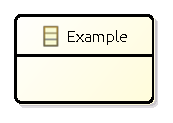
\includegraphics{images/05_library_of_transformations/02_type_level_transformations/01_regular_classes/class_type.pdf}
        \caption{$Tm_{Class}$ with $name = .\type{Example}$}
        \label{fig:library_of_transformations:type_level_transformations:regular_classes:visualisation:ecore}
    \end{subfigure}
    \begin{subfigure}{0.45\textwidth}
        \centering
        % To use this figure in your LaTeX document
% import the package groove/resources/groove2tikz.sty
%
\begin{tikzpicture}[scale=\tikzscale,name prefix=test-]
\node[type_node] (n0) at (0.950, -0.850) {\ml{\textbf{Example}}};

\end{tikzpicture}

        \caption{$TG_{Class}$ with $name = .\type{Example}$}
        \label{fig:library_of_transformations:type_level_transformations:regular_classes:visualisation:groove}
    \end{subfigure}
    \caption{Visualisation of the transformation of regular classes}
    \label{fig:library_of_transformations:type_level_transformations:regular_classes:visualisation}
\end{figure}

The first transformation that will be defined is a transformation of regular classes. A class without any additional properties is considered a regular class. The Ecore model for defining a regular class is given in the following definition:

\begin{defin}[Type model $Tm_{Class}$]
\label{defin:library_of_transformations:type_level_transformations:regular_classes:tmod_class}
Let $Tm_{Class}$ be the type model containing a regular class with identifier $name$. $Tm_{Class}$ is defined as:
\begin{align*}
Class =\ &\{name\} \\
Enum =\ &\{\} \\
UserDataType =\ &\{\} \\
Field =\ &\{\} \\
\mathrm{FieldSig} =\ &\{\} \\
EnumValue =\ &\{\} \\
Inh =\ &\{\} \\
Prop =\ &\{\} \\
Constant =\ &\{\} \\
\mathrm{ConstType} =\ &\{\}
\end{align*}
\isabellelref{tmod_class}{Ecore-GROOVE-Mapping-Library.ClassType}
\end{defin}

\begin{thm}[Correctness of $Tm_{Class}$]
\label{defin:library_of_transformations:type_level_transformations:regular_classes:tmod_class_correct}
$Tm_{Class}$ (\cref{defin:library_of_transformations:type_level_transformations:regular_classes:tmod_class}) is a consistent type model in the sense of \cref{defin:formalisations:ecore_formalisation:type_models:type_model_consistency}.
\isabellelref{tmod_class_correct}{Ecore-GROOVE-Mapping-Library.ClassType}
\end{thm}

A visual representation of $Tm_{Class}$ with identifier $.\type{Example}$ can be seen in \cref{fig:library_of_transformations:type_level_transformations:regular_classes:visualisation:ecore}. The correctness proof of $Tm_{Class}$ is trivial, and therefore not included here. The proof can be found as part of the Isabelle validated proofs.

In order to make composing transformation functions possible, $Tm_{Class}$ should be compatible with the type model it is combined with.

\begin{thm}[Correctness of $\mathrm{combine}(Tm, Tm_{Class})$]
\label{defin:library_of_transformations:type_level_transformations:regular_classes:tmod_class_combine_correct}
Assume a type model $Tm$ that is consistent in the sense of \cref{defin:formalisations:ecore_formalisation:type_models:type_model_consistency}. Then $Tm$ is compatible with $Tm_{Class}$ (in the sense of \cref{defin:transformation_framework:type_models_and_type_graphs:combining_type_models:compatibility}) if:
\begin{itemize}
    \item The identifier of the class in $Tm_{Class}$ is not yet an identifier for a class, enumeration type or user-defined data type in $Tm$;
    \item The identifier of the class in $Tm_{Class}$ is not in the namespace of any class, enumeration type or user-defined data type in $Tm$;
    \item None of the identifiers in any class, enumeration type or user-defined data type in $Tm$ is in the namespace of the class in $Tm_{Class}$.
\end{itemize}
\isabellelref{tmod_class_combine_correct}{Ecore-GROOVE-Mapping-Library.ClassType}
\end{thm}

\begin{proof}
Use \cref{defin:transformation_framework:type_models_and_type_graphs:combining_type_models:tmod_combine_merge_correct}. It is possible to show that all assumptions hold. Now we have shown that $\mathrm{combine}(Tm, Tm_{Class})$ is consistent in the sense of \cref{defin:formalisations:ecore_formalisation:type_models:type_model_consistency}.
\end{proof}

The definitions and theorems for a regular class within Ecore are now complete. 

\subsubsection{Encoding as node type}

A possible encoding for regular classes in Ecore is using a node type in GROOVE. This node type will get a transformed identifier as name. The encoding corresponding to $Tm_{Class}$ can then be represented as $TG_{Class}$, defined in the following definition:

\begin{defin}[Type graph $TG_{Class}$]
\label{defin:library_of_transformations:type_level_transformations:regular_classes:tg_class_as_node_type}
Let $TG_{Class}$ be the type graph containing a single node type which encodes a regular class $name$. $TG_{Class}$ is defined as:
\begin{align*}
NT =\ &\{\mathrm{ns\_\!to\_\!list}(name)\} \\
ET =\ &\{\} \\
\!\!\sqsubseteq\ =\ &\{( \mathrm{ns\_\!to\_\!list}(name), \mathrm{ns\_\!to\_\!list}(name) )\} \\
abs =\ &\{\} \\
\mathrm{mult} =\ &\{\} \\
contains =\ &\{\}
\end{align*}
\isabellelref{tg_class_as_node_type}{Ecore-GROOVE-Mapping-Library.ClassType}
\end{defin}

\begin{thm}[Correctness of $TG_{Class}$]
\label{defin:library_of_transformations:type_level_transformations:regular_classes:tg_class_as_node_type_correct}
$TG_{Class}$ (\cref{defin:library_of_transformations:type_level_transformations:regular_classes:tg_class_as_node_type}) is a valid type graph in the sense of \cref{defin:formalisations:groove_formalisation:type_graphs:type_graph_validity}.
\isabellelref{tg_class_as_node_type_correct}{Ecore-GROOVE-Mapping-Library.ClassType}
\end{thm}

A visual representation of $TG_{Class}$ with identifier $.\type{Example}$ can be seen in \cref{fig:library_of_transformations:type_level_transformations:regular_classes:visualisation:groove}. The correctness proof of $TG_{Class}$ is trivial, and therefore not included here. The proof can be found as part of the Isabelle validated proofs.

In order to make composing transformation functions possible, $TG_{Class}$ should be compatible with the type graph it is combined with.

\begin{thm}[Correctness of $\mathrm{combine}(TG, TG_{Class})$]
\label{defin:library_of_transformations:type_level_transformations:regular_classes:tg_class_as_node_type_combine_correct}
Assume a type graph $TG$ that is valid in the sense of \cref{defin:formalisations:groove_formalisation:type_graphs:type_graph_validity}. Then $TG$ is compatible with $TG_{Class}$ (in the sense of \cref{defin:transformation_framework:type_models_and_type_graphs:combining_type_graphs:compatibility}) if:
\begin{itemize}
    \item The node type of the encoded class in $TG_{Class}$ is not a node type in $TG$.
\end{itemize}
\isabellelref{tg_class_as_node_type_combine_correct}{Ecore-GROOVE-Mapping-Library.ClassType}
\end{thm}

\begin{proof}
Use \cref{defin:transformation_framework:type_models_and_type_graphs:combining_type_graphs:tg_combine_merge_correct}. It is possible to show that all assumptions hold. Now we have shown that $\mathrm{combine}(TG, TG_{Class})$ is valid in the sense of \cref{defin:formalisations:groove_formalisation:type_graphs:type_graph_validity}.
\end{proof}

The next definitions define the transformation function from $Tm_{Class}$ to $TG_{Class}$:

\begin{defin}[Transformation function $f_{Class}$]
\label{defin:library_of_transformations:type_level_transformations:regular_classes:tmod_class_to_tg_class_as_node_type}
The transformation function $f_{Class}(Tm)$ is defined as:
\begin{align*}
NT =\ &\{\mathrm{ns\_\!to\_\!list}(c) \mid c \in Class_{Tm}\} \\
ET =\ &\{\} \\
\!\!\sqsubseteq\ =\ &\{( \mathrm{ns\_\!to\_\!list}(c_1), \mathrm{ns\_\!to\_\!list}(c_2) ) \mid c_1 \in Class_{Tm} \land c_2 \in Class_{Tm} \} \\
abs =\ &\{\} \\
\mathrm{mult} =\ &\{\} \\
contains =\ &\{\}
\end{align*}
\isabellelref{tmod_class_to_tg_class_as_node_type}{Ecore-GROOVE-Mapping-Library.ClassType}
\end{defin}

\begin{thm}[Correctness of $f_{Class}$]
\label{defin:library_of_transformations:type_level_transformations:regular_classes:tmod_class_to_tg_class_as_node_type_func}
$f_{Class}(Tm)$ (\cref{defin:library_of_transformations:type_level_transformations:regular_classes:tmod_class_to_tg_class_as_node_type}) is a valid transformation function in the sense of \cref{defin:transformation_framework:type_models_and_type_graphs:combining_transformation_functions:transformation_function_type_model_type_graph} transforming $Tm_{Class}$ into $TG_{Class}$.
\isabellelref{tmod_class_to_tg_class_as_node_type_func}{Ecore-GROOVE-Mapping-Library.ClassType}
\end{thm}

The proof of the correctness of $f_{Class}$ will not be included here. Instead, it can be found in the validated Isabelle theories.

Finally, to complete the transformation, the transformation function that transforms $TG_{Class}$ into $Tm_{Class}$ is defined:

\begin{defin}[Transformation function $f'_{Class}$]
\label{defin:library_of_transformations:type_level_transformations:regular_classes:tg_class_as_node_type_to_tmod_class}
The transformation function $f'_{Class}(TG)$ is defined as:
\begin{align*}
Class =\ &\{\mathrm{list\_\!to\_\!ns}(n) \mid n \in NT_{TG}\} \\
Enum =\ &\{\} \\
UserDataType =\ &\{\} \\
Field =\ &\{\} \\
\mathrm{FieldSig} =\ &\{\} \\
EnumValue =\ &\{\} \\
Inh =\ &\{\} \\
Prop =\ &\{\} \\
Constant =\ &\{\} \\
\mathrm{ConstType} =\ &\{\}
\end{align*}
\isabellelref{tg_class_as_node_type_to_tmod_class}{Ecore-GROOVE-Mapping-Library.ClassType}
\end{defin}

\begin{thm}[Correctness of $f'_{Class}$]
\label{defin:library_of_transformations:type_level_transformations:regular_classes:tg_class_as_node_type_to_tmod_class_func}
$f'_{Class}(TG)$ (\cref{defin:library_of_transformations:type_level_transformations:regular_classes:tg_class_as_node_type_to_tmod_class}) is a valid transformation function in the sense of \cref{defin:transformation_framework:type_models_and_type_graphs:combining_transformation_functions:transformation_function_type_graph_type_model} transforming $TG_{Class}$ into $Tm_{Class}$.
\isabellelref{tg_class_as_node_type_to_tmod_class_func}{Ecore-GROOVE-Mapping-Library.ClassType}
\end{thm}

Once more, the correctness proof is not included here but can be found in the validated Isabelle proofs of this thesis.
\subsection{Abstract classes}
\label{subsec:library_of_transformations:type_level_transformations:abstract_classes}

\begin{figure}[H]
    \centering
    \begin{subfigure}{0.45\textwidth}
        \centering
        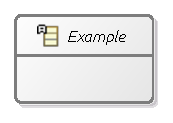
\includegraphics{images/05_library_of_transformations/02_type_level_transformations/02_abstract_classes/abstract_class_type.pdf}
        \caption{$Tm_{AbsClass}$ with $name = .\type{Example}$}
        \label{fig:library_of_transformations:type_level_transformations:abstract_classes:visualisation:ecore}
    \end{subfigure}
    \begin{subfigure}{0.45\textwidth}
        \centering
        % To use this figure in your LaTeX document
% import the package groove/resources/groove2tikz.sty
%
\begin{tikzpicture}[scale=\tikzscale,name prefix=test-]
\node[abstract_node] (n0) at (0.890, -0.830) {\ml{\textit{\textbf{Example}}}};

\end{tikzpicture}

        \caption{$TG_{AbsClass}$ with $name = .\type{Example}$}
        \label{fig:library_of_transformations:type_level_transformations:abstract_classes:visualisation:groove}
    \end{subfigure}
    \caption{Visualisation of the transformation of abstract classes}
    \label{fig:library_of_transformations:type_level_transformations:abstract_classes:visualisation}
\end{figure}

This section defines a transformation that is very close to the previous transformation. In this section, an abstract class without any additional properties is defined. The Ecore model for defining an abstract class is given in the following definition:

\begin{defin}[Type model $Tm_{AbsClass}$]
\label{defin:library_of_transformations:type_level_transformations:abstract_classes:tmod_abstract_class}
Let $Tm_{AbsClass}$ be the type model containing an abstract class with identifier $name$. $Tm_{AbsClass}$ is defined as:
\begin{align*}
Class =\ &\{name\} \\
Enum =\ &\{\} \\
UserDataType =\ &\{\} \\
Field =\ &\{\} \\
\mathrm{FieldSig} =\ &\{\} \\
EnumValue =\ &\{\} \\
Inh =\ &\{\} \\
Prop =\ &\{[ \type{abstract}, name ]\} \\
Constant =\ &\{\} \\
\mathrm{ConstType} =\ &\{\}
\end{align*}
\isabellelref{tmod_abstract_class}{Ecore-GROOVE-Mapping-Library.AbstractClassType}
\end{defin}

\begin{thm}[Correctness of $Tm_{AbsClass}$]
\label{defin:library_of_transformations:type_level_transformations:abstract_classes:tmod_abstract_class_correct}
$Tm_{AbsClass}$ (\cref{defin:library_of_transformations:type_level_transformations:abstract_classes:tmod_abstract_class}) is a consistent type model in the sense of \cref{defin:formalisations:ecore_formalisation:type_models:type_model_consistency}.
\isabellelref{tmod_abstract_class_correct}{Ecore-GROOVE-Mapping-Library.AbstractClassType}
\end{thm}

A visual representation of $Tm_{AbsClass}$ with identifier $.\type{Example}$ can be seen in \cref{fig:library_of_transformations:type_level_transformations:abstract_classes:visualisation:ecore}. The correctness proof of $Tm_{AbsClass}$ is trivial, and therefore not included here. The proof can be found as part of the Isabelle validated proofs.

In order to make composing transformation functions possible, $Tm_{AbsClass}$ should be compatible with the type model it is combined with.

\begin{thm}[Correctness of $\mathrm{combine}(Tm, Tm_{AbsClass})$]
\label{defin:library_of_transformations:type_level_transformations:abstract_classes:tmod_abstract_class_combine_correct}
Assume a type model $Tm$ that is consistent in the sense of \cref{defin:formalisations:ecore_formalisation:type_models:type_model_consistency}. Then $Tm$ is compatible with $Tm_{AbsClass}$ (in the sense of \cref{defin:transformation_framework:type_models_and_type_graphs:combining_type_models:compatibility}) if:
\begin{itemize}
    \item The identifier of the class in $Tm_{AbsClass}$ is not yet an identifier for a class, enumeration type or user-defined data type in $Tm$;
    \item The identifier of the class in $Tm_{AbsClass}$ is not in the namespace of any class, enumeration type or user-defined data type in $Tm$;
    \item None of the identifiers in any class, enumeration type or user-defined data type in $Tm$ is in the namespace of the class in $Tm_{AbsClass}$.
\end{itemize}
\isabellelref{tmod_abstract_class_combine_correct}{Ecore-GROOVE-Mapping-Library.AbstractClassType}
\end{thm}

\begin{proof}
Use \cref{defin:transformation_framework:type_models_and_type_graphs:combining_type_models:tmod_combine_merge_correct}. It is possible to show that all assumptions hold. Now we have shown that $\mathrm{combine}(Tm, Tm_{AbsClass})$ is consistent in the sense of \cref{defin:formalisations:ecore_formalisation:type_models:type_model_consistency}.
\end{proof}

The definitions and theorems for a regular class within Ecore are now complete. 

\subsubsection{Encoding as node type}

A possible encoding for abstract classes in Ecore is using a node type in GROOVE. This node type will get a transformed identifier as name. The encoding corresponding to $Tm_{AbsClass}$ can then be represented as $TG_{AbsClass}$, defined in the following definition:

\begin{defin}[Type graph $TG_{AbsClass}$]
\label{defin:library_of_transformations:type_level_transformations:abstract_classes:tg_abstract_class_as_node_type}
Let $TG_{AbsClass}$ be the type graph containing a single node type which encodes an abstract class $name$. $TG_{AbsClass}$ is defined as:
\begin{align*}
NT =\ &\{\mathrm{ns\_\!to\_\!list}(name)\} \\
ET =\ &\{\} \\
\!\!\sqsubseteq\ =\ &\{(\mathrm{ns\_\!to\_\!list}(name), \mathrm{ns\_\!to\_\!list}(name))\} \\
abs =\ &\{\mathrm{ns\_\!to\_\!list}(name)\} \\
\mathrm{mult} =\ &\{\} \\
contains =\ &\{\}
\end{align*}
\isabellelref{tg_abstract_class_as_node_type}{Ecore-GROOVE-Mapping-Library.AbstractClassType}
\end{defin}

\begin{thm}[Correctness of $TG_{Class}$]
\label{defin:library_of_transformations:type_level_transformations:abstract_classes:tg_abstract_class_as_node_type_correct}
$TG_{AbsClass}$ (\cref{defin:library_of_transformations:type_level_transformations:abstract_classes:tg_abstract_class_as_node_type}) is a valid type graph in the sense of \cref{defin:formalisations:groove_formalisation:type_graphs:type_graph_validity}.
\isabellelref{tg_abstract_class_as_node_type_correct}{Ecore-GROOVE-Mapping-Library.AbstractClassType}
\end{thm}

A visual representation of $TG_{AbsClass}$ with identifier $.\type{Example}$ can be seen in \cref{fig:library_of_transformations:type_level_transformations:abstract_classes:visualisation:groove}. The correctness proof of $TG_{AbsClass}$ is trivial, and therefore not included here. The proof can be found as part of the Isabelle validated proofs.

In order to make composing transformation functions possible, $TG_{AbsClass}$ should be compatible with the type graph it is combined with.

\begin{thm}[Correctness of $\mathrm{combine}(TG, TG_{AbsClass})$]
\label{defin:library_of_transformations:type_level_transformations:abstract_classes:tg_abstract_class_as_node_type_combine_correct}
Assume a type graph $TG$ that is valid in the sense of \cref{defin:formalisations:groove_formalisation:type_graphs:type_graph_validity}. Then $TG$ is compatible with $TG_{AbsClass}$ (in the sense of \cref{defin:transformation_framework:type_models_and_type_graphs:combining_type_graphs:compatibility}) if:
\begin{itemize}
    \item The node type of the encoded class in $TG_{AbsClass}$ is not a node type in $TG$.
\end{itemize}
\isabellelref{tg_abstract_class_as_node_type_combine_correct}{Ecore-GROOVE-Mapping-Library.AbstractClassType}
\end{thm}

\begin{proof}
Use \cref{defin:transformation_framework:type_models_and_type_graphs:combining_type_graphs:tg_combine_merge_correct}. It is possible to show that all assumptions hold. Now we have shown that $\mathrm{combine}(TG, TG_{AbsClass})$ is valid in the sense of \cref{defin:formalisations:groove_formalisation:type_graphs:type_graph_validity}.
\end{proof}

The next definitions define the transformation function from $Tm_{AbsClass}$ to $TG_{AbsClass}$:

\begin{defin}[Transformation function $f_{AbsClass}$]
\label{defin:library_of_transformations:type_level_transformations:abstract_classes:tmod_abstract_class_to_tg_abstract_class_as_node_type}
The transformation function $f_{AbsClass}(Tm)$ is defined as:
\begin{align*}
NT =\ &\{\mathrm{ns\_\!to\_\!list}(c) \mid c \in Class_{Tm}\} \\
ET =\ &\{\} \\
\!\!\sqsubseteq\ =\ &\{(\mathrm{ns\_\!to\_\!list}(c_1), \mathrm{ns\_\!to\_\!list}(c_2)) \mid c_1 \in Class_{Tm} \land c_2 \in Class_{Tm} \} \\
abs =\ &\{\mathrm{ns\_\!to\_\!list}(c) \mid c \in Class_{Tm}\} \\
\mathrm{mult} =\ &\{\} \\
contains =\ &\{\}
\end{align*}
\isabellelref{tmod_abstract_class_to_tg_abstract_class_as_node_type}{Ecore-GROOVE-Mapping-Library.AbstractClassType}
\end{defin}

\begin{thm}[Correctness of $f_{AbsClass}$]
\label{defin:library_of_transformations:type_level_transformations:abstract_classes:tmod_abstract_class_to_tg_abstract_class_as_node_type_func}
$f_{AbsClass}(Tm)$ (\cref{defin:library_of_transformations:type_level_transformations:abstract_classes:tmod_abstract_class_to_tg_abstract_class_as_node_type}) is a valid transformation function in the sense of \cref{defin:transformation_framework:type_models_and_type_graphs:combining_transformation_functions:transformation_function_type_model_type_graph} transforming $Tm_{AbsClass}$ into $TG_{AbsClass}$.
\isabellelref{tmod_abstract_class_to_tg_abstract_class_as_node_type_func}{Ecore-GROOVE-Mapping-Library.AbstractClassType}
\end{thm}

The proof of the correctness of $f_{AbsClass}$ will not be included here. Instead, it can be found in the validated Isabelle theories.

Finally, to complete the transformation, the transformation function that transforms $TG_{AbsClass}$ into $Tm_{AbsClass}$ is defined:

\begin{defin}[Transformation function $f'_{AbsClass}$]
\label{defin:library_of_transformations:type_level_transformations:abstract_classes:tg_abstract_class_as_node_type_to_tmod_abstract_class}
The transformation function $f'_{AbsClass}(TG)$ is defined as:
\begin{align*}
Class =\ &\{\mathrm{list\_\!to\_\!ns}(n) \mid n \in NT_{TG}\} \\
Enum =\ &\{\} \\
UserDataType =\ &\{\} \\
Field =\ &\{\} \\
\mathrm{FieldSig} =\ &\{\} \\
EnumValue =\ &\{\} \\
Inh =\ &\{\} \\
Prop =\ &\{[ \type{abstract}, \mathrm{ns\_\!to\_\!list}(c) ] \mid c \in Class_{Tm}\} \\
Constant =\ &\{\} \\
\mathrm{ConstType} =\ &\{\}
\end{align*}
\isabellelref{tg_abstract_class_as_node_type_to_tmod_abstract_class}{Ecore-GROOVE-Mapping-Library.AbstractClassType}
\end{defin}

\begin{thm}[Correctness of $f'_{AbsClass}$]
\label{defin:library_of_transformations:type_level_transformations:abstract_classes:tg_abstract_class_as_node_type_to_tmod_abstract_class_func}
$f'_{AbsClass}(TG)$ (\cref{defin:library_of_transformations:type_level_transformations:abstract_classes:tg_abstract_class_as_node_type_to_tmod_abstract_class}) is a valid transformation function in the sense of \cref{defin:transformation_framework:type_models_and_type_graphs:combining_transformation_functions:transformation_function_type_graph_type_model} transforming $TG_{AbsClass}$ into $Tm_{AbsClass}$.
\isabellelref{tg_abstract_class_as_node_type_to_tmod_abstract_class_func}{Ecore-GROOVE-Mapping-Library.AbstractClassType}
\end{thm}

Once more, the correctness proof is not included here but can be found in the validated Isabelle proofs of this thesis.
\subsection{Regular subclasses}
\label{subsec:library_of_transformations:type_level_transformations:regular_subclasses}

\begin{figure}[H]
    \centering
    \begin{subfigure}{0.4\textwidth}
        \centering
        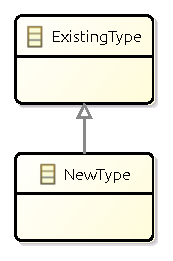
\includegraphics{images/05_library_of_transformations/02_type_level_transformations/03_regular_subclasses/class_subtype.pdf}
        \caption{$Tm_{Subclass}$ with $name = .\type{NewType}$ and $supertype = .\type{ExistingType}$}
        \label{fig:library_of_transformations:type_level_transformations:regular_subclasses:visualisation:ecore}
    \end{subfigure}
    \begin{subfigure}{0.4\textwidth}
        \centering
        % To use this figure in your LaTeX document
% import the package groove/resources/groove2tikz.sty
%
\begin{tikzpicture}[scale=\tikzscale,name prefix=test-]
\node[type_node] (n0) at (1.375, -1.525) {\ml{\textbf{NewType}}};
\node[type_node] (n1) at (1.365, -0.595) {\ml{\textbf{ExistingType}}};

\path[subtype_edge](n0.north -| 1.365, -0.595) --  (n1) ;
\end{tikzpicture}

        \caption{$TG_{Subclass}$ with $name = .\type{NewType}$ and $supertype = .\type{ExistingType}$}
        \label{fig:library_of_transformations:type_level_transformations:regular_subclasses:visualisation:groove}
    \end{subfigure}
    \caption{Visualisation of the transformation of regular subclasses}
    \label{fig:library_of_transformations:type_level_transformations:regular_subclasses:visualisation}
\end{figure}

This section will define the transformation of a regular subclass. Within this transformation, a newly introduced subclass is transformed, which extends an existing supertype. The Ecore type model that introduces such a subclass is defined as follows:

\begin{defin}[Type model $Tm_{Subclass}$]
\label{defin:library_of_transformations:type_level_transformations:regular_subclasses:tmod_subclass}
Let $Tm_{Subclass}$ be the type model containing a regular class with identifier $name$. The regular class $name$ extends another regular class with identifier $supertype$. Furthermore, $name \neq supertype$. $Tm_{Subclass}$ is defined as:
\begin{align*}
Class =\ &\{name, supertype\} \\
Enum =\ &\{\} \\
UserDataType =\ &\{\} \\
Field =\ &\{\} \\
\mathrm{FieldSig} =\ &\{\} \\
EnumValue =\ &\{\} \\
Inh =\ &\{(name, supertype)\} \\
Prop =\ &\{\} \\
Constant =\ &\{\} \\
\mathrm{ConstType} =\ &\{\}
\end{align*}
\isabellelref{tmod_subclass}{Ecore-GROOVE-Mapping-Library.SubclassType}
\end{defin}

\begin{thm}[Correctness of $Tm_{Subclass}$]
\label{defin:library_of_transformations:type_level_transformations:regular_subclasses:tmod_subclass_correct}
$Tm_{Subclass}$ (\cref{defin:library_of_transformations:type_level_transformations:regular_subclasses:tmod_subclass}) is a consistent type model in the sense of \cref{defin:formalisations:ecore_formalisation:type_models:type_model_consistency}.
\isabellelref{tmod_subclass_correct}{Ecore-GROOVE-Mapping-Library.SubclassType}
\end{thm}

A visual representation of $Tm_{Subclass}$ with the new subclass identified as $.\type{NewType}$ and the existing supertype identified as $.\type{ExistingType}$ can be seen in \cref{fig:library_of_transformations:type_level_transformations:regular_subclasses:visualisation:ecore}. The correctness proof of $Tm_{Subclass}$ is trivial, and therefore not included here. The proof can be found as part of the Isabelle validated proofs.

In order to make composing transformation functions possible, $Tm_{Subclass}$ should be compatible with the type model it is combined with.

\begin{thm}[Correctness of $\mathrm{combine}(Tm, Tm_{Subclass})$]
\label{defin:library_of_transformations:type_level_transformations:regular_subclasses:tmod_subclass_combine_correct}
Assume a type model $Tm$ that is consistent in the sense of \cref{defin:formalisations:ecore_formalisation:type_models:type_model_consistency}. Then $Tm$ is compatible with $Tm_{Subclass}$ (in the sense of \cref{defin:transformation_framework:type_models_and_type_graphs:combining_type_models:compatibility}) if:
\begin{itemize}
    \item The only shared type is the supertype, so $Class_{Tm} \cap Class_{Tm_{Subclass}} = \{ supertype \}$;
    \item The class $name$ is not in the namespace of class $supertype$, and vice versa;
    \item $name$ is not used as an identifier for an enumeration type or user-defined data type in $Tm$;
    \item The identifier of the class $name$ in $Tm_{Class}$ is not in the namespace of any class, enumeration type or user-defined data type in $Tm$;
    \item None of the identifiers in any class, enumeration type or user-defined data type in $Tm$ is in the namespace of the class $name$ in $Tm_{Class}$.
\end{itemize}
\isabellelref{tmod_subclass_combine_correct}{Ecore-GROOVE-Mapping-Library.SubclassType}
\end{thm}

\begin{proof}
Use \cref{defin:transformation_framework:type_models_and_type_graphs:combining_type_models:tmod_combine_merge_correct}. It is possible to show that all assumptions hold. For proving that the transitive closure of the inheritance relation is irreflexive, use the fact that $name$ only appears in the domain of the relation. Now we have shown that $\mathrm{combine}(Tm, Tm_{Class})$ is consistent in the sense of \cref{defin:formalisations:ecore_formalisation:type_models:type_model_consistency}.
\end{proof}

The definitions and theorems for a regular subclass within Ecore are now complete. 

\subsubsection{Encoding as node type}

A possible encoding for regular subclasses in Ecore is using node types in GROOVE. The supertype and newly introduced subtype will both be node types with their corresponding identifiers transformed. The encoding corresponding to $Tm_{Subclass}$ can then be represented as $TG_{Subclass}$, defined in the following definition:

\begin{defin}[Type graph $TG_{Subclass}$]
\label{defin:library_of_transformations:type_level_transformations:regular_subclasses:tg_subclass_as_node_type}
Let $TG_{Subclass}$ be a type graph containing a two node types. The first node type encodes the regular class $supertype$. The second node type encodes a regular class $name$ which extends the encoded class $supertype$. Furthermore $name \neq supertype$. $TG_{Subclass}$ is defined as:
\begin{align*}
NT =\ &\{\mathrm{ns\_\!to\_\!list}(name), \mathrm{ns\_\!to\_\!list}(supertype)\} \\
ET =\ &\{\} \\
\!\!\sqsubseteq\ =\ &\{
(\mathrm{ns\_\!to\_\!list}(name), \mathrm{ns\_\!to\_\!list}(name)), \\&
(\mathrm{ns\_\!to\_\!list}(supertype), \mathrm{ns\_\!to\_\!list}(supertype)), \\&
(\mathrm{ns\_\!to\_\!list}(name), \mathrm{ns\_\!to\_\!list}(supertype))
\} \\
abs =\ &\{\} \\
\mathrm{mult} =\ &\{\} \\
contains =\ &\{\}
\end{align*}
\isabellelref{tg_subclass_as_node_type}{Ecore-GROOVE-Mapping-Library.SubclassType}
\end{defin}

\begin{thm}[Correctness of $TG_{Subclass}$]
\label{defin:library_of_transformations:type_level_transformations:regular_subclasses:tg_subclass_as_node_type_correct}
$TG_{Subclass}$ (\cref{defin:library_of_transformations:type_level_transformations:regular_subclasses:tg_subclass_as_node_type}) is a valid type graph in the sense of \cref{defin:formalisations:groove_formalisation:type_graphs:type_graph_validity}.
\isabellelref{tg_subclass_as_node_type_correct}{Ecore-GROOVE-Mapping-Library.SubclassType}
\end{thm}

A visual representation of $TG_{Subclass}$ with the new subclass identified as $.\type{NewType}$ and the existing supertype identified as $.\type{ExistingType}$ both encoded as node type, is shown in \cref{fig:library_of_transformations:type_level_transformations:regular_subclasses:visualisation:groove}. The correctness proof of $TG_{Subclass}$ is trivial, and therefore not included here. The proof can be found as part of the Isabelle validated proofs.

In order to make composing transformation functions possible, $TG_{Subclass}$ should be compatible with the type graph it is combined with.

\begin{thm}[Correctness of $\mathrm{combine}(TG, TG_{Subclass})$]
\label{defin:library_of_transformations:type_level_transformations:regular_subclasses:tg_subclass_as_node_type_combine_correct}
Assume a type graph $TG$ that is valid in the sense of \cref{defin:formalisations:groove_formalisation:type_graphs:type_graph_validity}. Then $TG$ is compatible with $TG_{Subclass}$ (in the sense of \cref{defin:transformation_framework:type_models_and_type_graphs:combining_type_graphs:compatibility}) if:
\begin{itemize}
    \item The only shared node type in $TG$ and $TG_{Subclass}$ is the node type of the encoded supertype.
\end{itemize}
\isabellelref{tg_subclass_as_node_type_combine_correct}{Ecore-GROOVE-Mapping-Library.SubclassType}
\end{thm}

\begin{proof}
Use \cref{defin:transformation_framework:type_models_and_type_graphs:combining_type_graphs:tg_combine_merge_correct}. It is possible to show that all assumptions hold. For proving the antisymmetry of the inheritance relation, use the fact that the node type which encodes class $name$ only appears in the domain of the relation. Now we have shown that $\mathrm{combine}(TG, TG_{Subclass})$ is valid in the sense of \cref{defin:formalisations:groove_formalisation:type_graphs:type_graph_validity}.
\end{proof}

The next definitions define the transformation function from $Tm_{Sublass}$ to $TG_{Sublass}$:

\begin{defin}[Transformation function $f_{Subclass}$]
\label{defin:library_of_transformations:type_level_transformations:regular_subclasses:tmod_subclass_to_tg_subclass_as_node_type}
The transformation function $f_{Subclass}(Tm)$ is defined as:
\begin{align*}
NT =\ &\{\mathrm{ns\_\!to\_\!list}(c) \mid c \in Class_{Tm}\} \\
ET =\ &\{\} \\
\!\!\sqsubseteq\ =\ &\{(\mathrm{ns\_\!to\_\!list}(c_1), \mathrm{ns\_\!to\_\!list}(c_2)) \mid c_1 \in Class_{Tm} \land c_2 \in Class_{Tm} \land c_1 = c_2 \}\ \cup \\&
\{(\mathrm{ns\_\!to\_\!list}(i), \mathrm{ns\_\!to\_\!list}(j)) \mid (i, j) \in Inh_{Tm} \} \\
abs =\ &\{\} \\
\mathrm{mult} =\ &\{\} \\
contains =\ &\{\}
\end{align*}
\isabellelref{tmod_subclass_to_tg_subclass_as_node_type}{Ecore-GROOVE-Mapping-Library.SubclassType}
\end{defin}

\begin{thm}[Correctness of $f_{Subclass}$]
\label{defin:library_of_transformations:type_level_transformations:regular_subclasses:tmod_subclass_to_tg_subclass_as_node_type_func}
$f_{Subclass}(Tm)$ (\cref{defin:library_of_transformations:type_level_transformations:regular_subclasses:tmod_subclass_to_tg_subclass_as_node_type}) is a valid transformation function in the sense of \cref{defin:transformation_framework:type_models_and_type_graphs:combining_transformation_functions:transformation_function_type_model_type_graph} transforming $Tm_{Subclass}$ into $TG_{Subclass}$.
\isabellelref{tmod_subclass_to_tg_subclass_as_node_type_func}{Ecore-GROOVE-Mapping-Library.SubclassType}
\end{thm}

The proof of the correctness of $f_{Subclass}$ will not be included here. Instead, it can be found in the validated Isabelle theories.

Finally, to complete the transformation, the transformation function that transforms $TG_{Subclass}$ into $Tm_{Subclass}$ is defined:

\begin{defin}[Transformation function $f'_{Subclass}$]
\label{defin:library_of_transformations:type_level_transformations:regular_subclasses:tg_subclass_as_node_type_to_tmod_subclass}
The transformation function $f'_{Subclass}(TG)$ is defined as:
\begin{align*}
Class =\ &\{\mathrm{list\_\!to\_\!ns}(n) \mid n \in NT_{TG}\} \\
Enum =\ &\{\} \\
UserDataType =\ &\{\} \\
Field =\ &\{\} \\
\mathrm{FieldSig} =\ &\{\} \\
EnumValue =\ &\{\} \\
Inh =\ &\{(\mathrm{list\_\!to\_\!ns}(i), \mathrm{list\_\!to\_\!ns}(j)) \mid (i, j) \in\ \sqsubseteq_{TG} \land\ i \neq j \} \\
Prop =\ &\{\} \\
Constant =\ &\{\} \\
\mathrm{ConstType} =\ &\{\}
\end{align*}
\isabellelref{tg_subclass_as_node_type_to_tmod_subclass}{Ecore-GROOVE-Mapping-Library.SubclassType}
\end{defin}

\begin{thm}[Correctness of $f'_{Subclass}$]
\label{defin:library_of_transformations:type_level_transformations:regular_subclasses:tg_subclass_as_node_type_to_tmod_subclass_func}
$f'_{Subclass}(TG)$ (\cref{defin:library_of_transformations:type_level_transformations:regular_subclasses:tg_subclass_as_node_type_to_tmod_subclass}) is a valid transformation function in the sense of \cref{defin:transformation_framework:type_models_and_type_graphs:combining_transformation_functions:transformation_function_type_graph_type_model} transforming $TG_{Subclass}$ into $Tm_{Subclass}$.
\isabellelref{tg_subclass_as_node_type_to_tmod_subclass_func}{Ecore-GROOVE-Mapping-Library.SubclassType}
\end{thm}

Once more, the correctness proof is not included here but can be found in the validated Isabelle proofs of this thesis.
\subsection{Enumeration types}
\label{subsec:library_of_transformations:type_level_transformations:enumeration_types}

\begin{figure}[H]
    \centering
    \begin{subfigure}{0.25\textwidth}
        \centering
        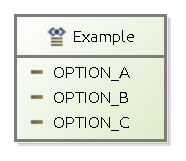
\includegraphics{images/05_library_of_transformations/02_type_level_transformations/04_enumeration_types/enum_type.pdf}
        \caption{$Tm_{Enum}$ with \\$name = .\type{Example}$ and \\$values = \{ \type{OPTION\_A},$\\$ \type{OPTION\_B}, \type{OPTION\_C} \}$}
        \label{fig:library_of_transformations:type_level_transformations:enumeration_types:visualisation:ecore}
    \end{subfigure}
    \\
    \begin{subfigure}{0.65\textwidth}
        \centering
        % To use this figure in your LaTeX document
% import the package groove/resources/groove2tikz.sty
%
\begin{tikzpicture}[scale=\tikzscale,name prefix=test-]
\node[abstract_node] (n1) at (3.160, -0.665) {\ml{\textit{\textbf{Example}}}};
\node[type_node] (n0) at (1.550, -1.875) {\ml{\textbf{Example\$OPTION\_A}}};
\node[type_node] (n2) at (3.160, -1.875) {\ml{\textbf{Example\$OPTION\_B}}};
\node[type_node] (n3) at (4.760, -1.875) {\ml{\textbf{Example\$OPTION\_C}}};

\path[subtype_edge] (n0)  --  (n1) ;
\path[subtype_edge](n2.north -| 3.160, -0.665) --  (n1) ;
\path[subtype_edge] (n3)  --  (n1) ;
\end{tikzpicture}

        \caption{$TG_{EnumNodes}$ with $name = .\type{Example}$ and\\$values = \{ \type{OPTION\_A}, \type{OPTION\_B}, \type{OPTION\_C} \}$}
        \label{fig:library_of_transformations:type_level_transformations:enumeration_types:visualisation:groove_nodes}
    \end{subfigure}
    \begin{subfigure}{0.25\textwidth}
        \centering
        % To use this figure in your LaTeX document
% import the package groove/resources/groove2tikz.sty
%
\begin{tikzpicture}[scale=\tikzscale,name prefix=test-]
\node[type_node] (n1) at (3.160, -0.665) {\ml{\textbf{Example}\\\textit{OPTION\_A}\\\textit{OPTION\_B}\\\textit{OPTION\_C}}};

\end{tikzpicture}

        \caption{$TG_{EnumFlags}$ with \\$name = .\type{Example}$ and \\$values = \{ \type{OPTION\_A},$\\$ \type{OPTION\_B}, \type{OPTION\_C} \}$}
        \label{fig:library_of_transformations:type_level_transformations:enumeration_types:visualisation:groove_flags}
    \end{subfigure}
    \caption{Visualisations of the transformations of enumeration types}
    \label{fig:library_of_transformations:type_level_transformations:enumeration_types:visualisation}
\end{figure}

This section will define the transformation of an enumeration type. Within this transformation, a new enumeration type is introduced, including its possible values. The Ecore type model that introduces such a subclass is defined as follows:

\begin{defin}[Type model $Tm_{Enum}$]
\label{defin:library_of_transformations:type_level_transformations:enumeration_types:tmod_enum}
Let $Tm_{Enum}$ be the type model containing a enumeration type with identifier $name$. The values of this enumeration type are defined as part of sequence $values$. $Tm_{Enum}$ is defined as:
\begin{align*}
Class =\ &\{\} \\
Enum =\ &\{name\} \\
UserDataType =\ &\{\} \\
Field =\ &\{\} \\
\mathrm{FieldSig} =\ &\{\} \\
EnumValue =\ &\{ (name, v) \mid v \in values \} \\
Inh =\ &\{\} \\
Prop =\ &\{\} \\
Constant =\ &\{\} \\
\mathrm{ConstType} =\ &\{\}
\end{align*}
\isabellelref{tmod_enum}{Ecore-GROOVE-Mapping-Library.EnumType}
\end{defin}

\begin{thm}[Correctness of $Tm_{Enum}$]
\label{defin:library_of_transformations:type_level_transformations:enumeration_types:tmod_enum_correct}
$Tm_{Subclass}$ (\cref{defin:library_of_transformations:type_level_transformations:enumeration_types:tmod_enum}) is a consistent type model in the sense of \cref{defin:formalisations:ecore_formalisation:type_models:type_model_consistency}.
\isabellelref{tmod_enum_correct}{Ecore-GROOVE-Mapping-Library.EnumType}
\end{thm}

A visual representation of $Tm_{Enum}$ with $.\type{Example}$ as identifier for the new enumeration type and $\type{OPTION\_A}$, $\type{OPTION\_B}$ and $\type{OPTION\_C}$ as its values can be seen in \cref{fig:library_of_transformations:type_level_transformations:enumeration_types:visualisation:ecore}. The correctness proof of $Tm_{Enum}$ is trivial, and therefore not included here. The proof can be found as part of the Isabelle validated proofs.

In order to make composing transformation functions possible, $Tm_{Enum}$ should be compatible with the type model it is combined with.

\begin{thm}[Correctness of $\mathrm{combine}(Tm, Tm_{Enum})$]
\label{defin:library_of_transformations:type_level_transformations:enumeration_types:tmod_enum_combine_correct}
Assume a type model $Tm$ that is consistent in the sense of \cref{defin:formalisations:ecore_formalisation:type_models:type_model_consistency}. Then $Tm$ is compatible with $Tm_{Enum}$ (in the sense of \cref{defin:transformation_framework:type_models_and_type_graphs:combining_type_models:compatibility}) if:
\begin{itemize}
    \item The identifier of the enumeration type in $Tm_{Enum}$ is not yet an identifier for a class, enumeration type or user-defined data type in $Tm$;
    \item The identifier of the enumeration type in $Tm_{Enum}$ is not in the namespace of any class, enumeration type or user-defined data type in $Tm$;
    \item None of the identifiers in any class, enumeration type or user-defined data type in $Tm$ is in the namespace of the enumeration type in $Tm_{Enum}$.
\end{itemize}
\isabellelref{tmod_enum_combine_correct}{Ecore-GROOVE-Mapping-Library.EnumType}
\end{thm}

\begin{proof}
Use \cref{defin:transformation_framework:type_models_and_type_graphs:combining_type_models:tmod_combine_merge_correct}. It is possible to show that all assumptions hold. Now we have shown that $\mathrm{combine}(Tm, Tm_{Enum})$ is consistent in the sense of \cref{defin:formalisations:ecore_formalisation:type_models:type_model_consistency}.
\end{proof}

The definitions and theorems for a regular subclass within Ecore are now complete. 

\subsubsection{Encoding as node type}

A possible encoding for enumeration types in Ecore is using node types in GROOVE. In this case, the enumeration type itself is transformed into an abstract node type. Each value of the enumeration type is converted to its own node type, extending the abstract node type. The encoding corresponding to $Tm_{Enum}$ can then be represented as $TG_{EnumNodes}$, defined in the following definition:

\begin{defin}[Type graph $TG_{EnumNodes}$]
\label{defin:library_of_transformations:type_level_transformations:enumeration_types:tg_enum_as_node_types}
Let $TG_{EnumNodes}$ be a type graph containing multiple node types. The first node type encodes the enumeration type $name$. The other node types encode the $values$ of enumeration type $name$. $TG_{EnumNodes}$ is defined as:
\begin{align*}
NT =\ &\{\mathrm{ns\_\!to\_\!list}(name)\} \cup \{ \mathrm{ns\_\!to\_\!list}(name) \append \langle v \rangle \mid v \in values \} \\
ET =\ &\{\} \\
\!\!\sqsubseteq\ =\ &\{(\mathrm{ns\_\!to\_\!list}(name), \mathrm{ns\_\!to\_\!list}(name))\}\ \cup \\&
\{(\mathrm{ns\_\!to\_\!list}(name) \append \langle v \rangle, \mathrm{ns\_\!to\_\!list}(name) \append \langle v \rangle) \mid v \in values \}\ \cup \\&
\{(\mathrm{ns\_\!to\_\!list}(name) \append \langle v \rangle, \mathrm{ns\_\!to\_\!list}(name)) \mid v \in values \} \\
abs =\ &\{\mathrm{ns\_\!to\_\!list}(name)\} \\
\mathrm{mult} =\ &\{\} \\
contains =\ &\{\}
\end{align*}
\isabellelref{tg_enum_as_node_types}{Ecore-GROOVE-Mapping-Library.EnumType}
\end{defin}

\begin{thm}[Correctness of $TG_{EnumNodes}$]
\label{defin:library_of_transformations:type_level_transformations:enumeration_types:tg_enum_as_node_types_correct}
$TG_{EnumNodes}$ (\cref{defin:library_of_transformations:type_level_transformations:enumeration_types:tg_enum_as_node_types}) is a valid type graph in the sense of \cref{defin:formalisations:groove_formalisation:type_graphs:type_graph_validity}.
\isabellelref{tg_enum_as_node_types_correct}{Ecore-GROOVE-Mapping-Library.EnumType}
\end{thm}

A visual representation of $TG_{EnumNodes}$ with $.\type{Example}$ as identifier for the encoded enumeration type and $\type{OPTION\_A}$, $\type{OPTION\_B}$ and $\type{OPTION\_C}$ as its values can be seen in \cref{fig:library_of_transformations:type_level_transformations:enumeration_types:visualisation:groove_nodes}. Please note that in this visualisation, the sequences are concatenated using the dollar sign $\$$. The correctness proof of $TG_{EnumNodes}$ is trivial, and therefore not included here. The proof can be found as part of the Isabelle validated proofs.

In order to make composing transformation functions possible, $TG_{EnumNodes}$ should be compatible with the type graph it is combined with.

\begin{thm}[Correctness of $\mathrm{combine}(TG, TG_{EnumNodes})$]
\label{defin:library_of_transformations:type_level_transformations:enumeration_types:tg_enum_as_node_types_combine_correct}
Assume a type graph $TG$ that is valid in the sense of \cref{defin:formalisations:groove_formalisation:type_graphs:type_graph_validity}. Then $TG$ is compatible with $TG_{EnumNodes}$ (in the sense of \cref{defin:transformation_framework:type_models_and_type_graphs:combining_type_graphs:compatibility}) if:
\begin{itemize}
    \item There are no shared node types between $TG_{EnumNodes}$ and $TG$.
\end{itemize}
\isabellelref{tg_enum_as_node_types_combine_correct}{Ecore-GROOVE-Mapping-Library.EnumType}
\end{thm}

\begin{proof}
Use \cref{defin:transformation_framework:type_models_and_type_graphs:combining_type_graphs:tg_combine_merge_correct}. It is possible to show that all assumptions hold. Now we have shown that $\mathrm{combine}(TG, TG_{EnumNodes})$ is valid in the sense of \cref{defin:formalisations:groove_formalisation:type_graphs:type_graph_validity}.
\end{proof}

The next definitions define the transformation function from $Tm_{Enum}$ to $TG_{EnumNodes}$:

\begin{defin}[Transformation function $f_{EnumNodes}$]
\label{defin:library_of_transformations:type_level_transformations:enumeration_types:tmod_enum_to_tg_enum_as_node_types}
The transformation function $f_{EnumNodes}(Tm)$ is defined as:
\begin{align*}
NT =\ &\{\mathrm{ns\_\!to\_\!list}(e) \mid e \in Enum_{Tm}\} \cup \{\mathrm{ns\_\!to\_\!list}(e) \append \langle v \rangle \mid (e, v) \in EnumValue_{Tm}\} \\
ET =\ &\{\} \\
\!\!\sqsubseteq\ =\ &\{(\mathrm{ns\_\!to\_\!list}(e_1), \mathrm{ns\_\!to\_\!list}(e_2)) \mid e_1 \in Enum_{Tm} \land e_2 \in Enum_{Tm} \}\ \cup \\&
\{(\mathrm{ns\_\!to\_\!list}(i) \append \langle j \rangle, \mathrm{ns\_\!to\_\!list}(i) \append \langle j \rangle) \mid (i, j) \in EnumValue_{Tm} \}\ \cup \\&
\{(\mathrm{ns\_\!to\_\!list}(i) \append \langle j \rangle, \mathrm{ns\_\!to\_\!list}(e)) \mid (i, j) \in EnumValue_{Tm} \land e \in Enum_{Tm} \} \\
abs =\ &\{\} \\
\mathrm{mult} =\ &\{\} \\
contains =\ &\{\}
\end{align*}
\isabellelref{tmod_enum_to_tg_enum_as_node_types}{Ecore-GROOVE-Mapping-Library.EnumType}
\end{defin}

\begin{thm}[Correctness of $f_{EnumNodes}$]
\label{defin:library_of_transformations:type_level_transformations:enumeration_types:tmod_enum_to_tg_enum_as_node_types_func}
$f_{EnumNodes}(Tm)$ (\cref{defin:library_of_transformations:type_level_transformations:enumeration_types:tmod_enum_to_tg_enum_as_node_types}) is a valid transformation function in the sense of \cref{defin:transformation_framework:type_models_and_type_graphs:combining_transformation_functions:transformation_function_type_model_type_graph} transforming $Tm_{Enum}$ into $TG_{EnumNodes}$.
\isabellelref{tmod_enum_to_tg_enum_as_node_types_func}{Ecore-GROOVE-Mapping-Library.EnumType}
\end{thm}

The proof of the correctness of $f_{EnumNodes}$ will not be included here. Instead, it can be found in the validated Isabelle theories.

Finally, to complete the transformation, the transformation function that transforms $TG_{EnumNodes}$ into $Tm_{Enum}$ is defined:

\begin{defin}[Transformation function $f'_{EnumNodes}$]
\label{defin:library_of_transformations:type_level_transformations:enumeration_types:tg_enum_as_node_types_to_tmod_enum}
The transformation function $f'_{EnumNodes}(TG, name)$ is defined as:
\begin{align*}
Class =\ &\{\} \\
Enum =\ &\{\mathrm{list\_\!to\_\!ns}(n) \mid n \in NT_{TG} \land n = \mathrm{id\_\!to\_\!name}(name)\} \\
UserDataType =\ &\{\} \\
Field =\ &\{\} \\
\mathrm{FieldSig} =\ &\{\} \\
EnumValue =\ &\{(\mathrm{list\_\!to\_\!ns}(e), v) \mid e \append \langle v \rangle \in NT_{TG} \land e \append \langle v \rangle \neq \mathrm{id\_\!to\_\!name}(name) \} \\
Inh =\ &\{\} \\
Prop =\ &\{\} \\
Constant =\ &\{\} \\
\mathrm{ConstType} =\ &\{\}
\end{align*}
\isabellelref{tg_enum_as_node_types_to_tmod_enum}{Ecore-GROOVE-Mapping-Library.EnumType}
\end{defin}

\begin{thm}[Correctness of $f'_{EnumNodes}$]
\label{defin:library_of_transformations:type_level_transformations:enumeration_types:tg_enum_as_node_types_to_tmod_enum_func}
$f'_{EnumNodes}(TG, name)$ (\cref{defin:library_of_transformations:type_level_transformations:enumeration_types:tg_enum_as_node_types_to_tmod_enum}) is a valid transformation function in the sense of \cref{defin:transformation_framework:type_models_and_type_graphs:combining_transformation_functions:transformation_function_type_graph_type_model} transforming $TG_{EnumNodes}$ into $Tm_{Enum}$.
\isabellelref{tg_enum_as_node_types_to_tmod_enum_func}{Ecore-GROOVE-Mapping-Library.EnumType}
\end{thm}

Once more, the correctness proof is not included here but can be found in the validated Isabelle proofs of this thesis.

\subsubsection{Encoding as flags}

Another possible encoding for enumeration types in Ecore is using flags in GROOVE. In this case, the enumeration type itself is transformed into a regular node type. Each value of the enumeration type is converted to a flag on this node type. The encoding corresponding to $Tm_{Enum}$ can then be represented as $TG_{EnumFlags}$, defined in the following definition:

\begin{defin}[Type graph $TG_{EnumFlags}$]
\label{defin:library_of_transformations:type_level_transformations:enumeration_types:tg_enum_as_flags}
Let $TG_{EnumFlags}$ be a type graph containing a single node type which encodes the enumeration type $name$. The flags on the node type of $name$ encode the different $values$. $TG_{EnumFlags}$ is defined as:
\begin{align*}
NT =\ &\{\mathrm{ns\_\!to\_\!list}(name)\} \\
ET =\ &\{ (\mathrm{ns\_\!to\_\!list}(name), \langle v \rangle, \mathrm{ns\_\!to\_\!list}(name)) \mid v \in values \}\\
\!\!\sqsubseteq\ =\ &\{(\mathrm{ns\_\!to\_\!list}(name), \mathrm{ns\_\!to\_\!list}(name))\} \\
abs =\ &\{\} \\
\mathrm{mult}(e) =\ &\begin{cases}
    (0..1, 0..1) &\mathrm{if}\ e \in ET_{TG_{EnumFlags}}
\end{cases}\\
contains =\ &\{\}
\end{align*}
\isabellelref{tg_enum_as_flags}{Ecore-GROOVE-Mapping-Library.EnumType}
\end{defin}

\begin{thm}[Correctness of $TG_{EnumFlags}$]
\label{defin:library_of_transformations:type_level_transformations:enumeration_types:tg_enum_as_flags_correct}
$TG_{EnumFlags}$ (\cref{defin:library_of_transformations:type_level_transformations:enumeration_types:tg_enum_as_flags}) is a valid type graph in the sense of \cref{defin:formalisations:groove_formalisation:type_graphs:type_graph_validity}.
\isabellelref{tg_enum_as_flags_correct}{Ecore-GROOVE-Mapping-Library.EnumType}
\end{thm}

A visual representation of $TG_{EnumFlags}$ with $.\type{Example}$ as identifier for the encoded enumeration type and $\type{OPTION\_A}$, $\type{OPTION\_B}$ and $\type{OPTION\_C}$ as its values can be seen in \cref{fig:library_of_transformations:type_level_transformations:enumeration_types:visualisation:groove_flags}. The correctness proof of $TG_{EnumFlags}$ is trivial, and therefore not included here. The proof can be found as part of the Isabelle validated proofs.

In order to make composing transformation functions possible, $TG_{EnumFlags}$ should be compatible with the type graph it is combined with.

\begin{thm}[Correctness of $\mathrm{combine}(TG, TG_{EnumFlags})$]
\label{defin:library_of_transformations:type_level_transformations:enumeration_types:tg_enum_as_flags_combine_correct}
Assume a type graph $TG$ that is valid in the sense of \cref{defin:formalisations:groove_formalisation:type_graphs:type_graph_validity}. Then $TG$ is compatible with $TG_{EnumFlags}$ (in the sense of \cref{defin:transformation_framework:type_models_and_type_graphs:combining_type_graphs:compatibility}) if:
\begin{itemize}
    \item There are no shared node types between $TG_{EnumFlags}$ and $TG$.
\end{itemize}
\isabellelref{tg_enum_as_flags_combine_correct}{Ecore-GROOVE-Mapping-Library.EnumType}
\end{thm}

\begin{proof}
Use \cref{defin:transformation_framework:type_models_and_type_graphs:combining_type_graphs:tg_combine_merge_correct}. It is possible to show that all assumptions hold. Now we have shown that $\mathrm{combine}(TG, TG_{EnumFlags})$ is valid in the sense of \cref{defin:formalisations:groove_formalisation:type_graphs:type_graph_validity}.
\end{proof}

The next definitions define the transformation function from $Tm_{Enum}$ to $TG_{EnumFlags}$:

\begin{defin}[Transformation function $f_{EnumFlags}$]
\label{defin:library_of_transformations:type_level_transformations:enumeration_types:tmod_enum_to_tg_enum_as_flags}
The transformation function $f_{EnumFlags}(Tm)$ is defined as:
\begin{align*}
NT =\ &\{\mathrm{ns\_\!to\_\!list}(e) \mid e \in Enum_{Tm}\} \\
ET =\ &\{(\mathrm{ns\_\!to\_\!list}(e), v, \mathrm{ns\_\!to\_\!list}(e)) \mid (e, v) \in EnumValue_{Tm}\} \\
\!\!\sqsubseteq\ =\ &\{(\mathrm{ns\_\!to\_\!list}(e_1), \mathrm{ns\_\!to\_\!list}(e_2)) \mid e_1 \in Enum_{Tm} \land e_2 \in Enum_{Tm} \} \\
abs =\ &\{\} \\
\mathrm{mult}(e) =\ &\begin{cases}
    (0..1, 0..1) &\mathrm{if}\ e \in \{(\mathrm{ns\_\!to\_\!list}(n), v, \mathrm{ns\_\!to\_\!list}(n)) \mid (n, v) \in EnumValue_{Tm}\}
\end{cases}\\
contains =\ &\{\}
\end{align*}
\isabellelref{tmod_enum_to_tg_enum_as_flags}{Ecore-GROOVE-Mapping-Library.EnumType}
\end{defin}

\begin{thm}[Correctness of $f_{EnumFlags}$]
\label{defin:library_of_transformations:type_level_transformations:enumeration_types:tmod_enum_to_tg_enum_as_flags_func}
$f_{EnumFlags}(Tm)$ (\cref{defin:library_of_transformations:type_level_transformations:enumeration_types:tmod_enum_to_tg_enum_as_flags}) is a valid transformation function in the sense of \cref{defin:transformation_framework:type_models_and_type_graphs:combining_transformation_functions:transformation_function_type_model_type_graph} transforming $Tm_{Enum}$ into $TG_{EnumFlags}$.
\isabellelref{tmod_enum_to_tg_enum_as_flags_func}{Ecore-GROOVE-Mapping-Library.EnumType}
\end{thm}

The proof of the correctness of $f_{EnumFlags}$ will not be included here. Instead, it can be found in the validated Isabelle theories.

Finally, to complete the transformation, the transformation function that transforms $TG_{EnumFlags}$ into $Tm_{Enum}$ is defined:

\begin{defin}[Transformation function $f'_{EnumFlags}$]
\label{defin:library_of_transformations:type_level_transformations:enumeration_types:tg_enum_as_flags_to_tmod_enum}
The transformation function $f'_{EnumFlags}(TG)$ is defined as:
\begin{align*}
Class =\ &\{\} \\
Enum =\ &\{\mathrm{list\_\!to\_\!ns}(n) \mid n \in NT_{TG}\} \\
UserDataType =\ &\{\} \\
Field =\ &\{\} \\
\mathrm{FieldSig} =\ &\{\} \\
EnumValue =\ &\{(\mathrm{list\_\!to\_\!ns}(e), v) \mid (e, v, e) \in ET_{TG} \} \\
Inh =\ &\{\} \\
Prop =\ &\{\} \\
Constant =\ &\{\} \\
\mathrm{ConstType} =\ &\{\}
\end{align*}
\isabellelref{tg_enum_as_flags_to_tmod_enum}{Ecore-GROOVE-Mapping-Library.EnumType}
\end{defin}

\begin{thm}[Correctness of $f'_{EnumNodes}$]
\label{defin:library_of_transformations:type_level_transformations:enumeration_types:tg_enum_as_flags_to_tmod_enum_func}
$f'_{EnumFlags}(TG)$ (\cref{defin:library_of_transformations:type_level_transformations:enumeration_types:tg_enum_as_flags_to_tmod_enum}) is a valid transformation function in the sense of \cref{defin:transformation_framework:type_models_and_type_graphs:combining_transformation_functions:transformation_function_type_graph_type_model} transforming $TG_{EnumFlags}$ into $Tm_{Enum}$.
\isabellelref{tg_enum_as_flags_to_tmod_enum_func}{Ecore-GROOVE-Mapping-Library.EnumType}
\end{thm}

Once more, the correctness proof is not included here but can be found in the validated Isabelle proofs of this thesis.
\subsection{User-defined data types}
\label{subsec:library_of_transformations:instance_level_transformations:user_defined_data_types}

In this section, the instance level transformation corresponding to the type level transformation of user-defined data types is discussed. The type level transformation of user-defined data types can be found in \cref{subsec:library_of_transformations:type_level_transformations:user_defined_data_types}.

This definition does not actually introduce values for user-defined data types. This is done upon instantiating the type via a field. Therefore, an empty instance model and empty instance graph will be used for completeness.

First, the corresponding instance model is introduced.

\begin{defin}[Instance model $Im_{UserType}$]
\label{defin:library_of_transformations:instance_level_transformations:user_defined_data_types:imod_userdatatype}
Let $Im_{UserType}$ be the empty instance model $Im_\epsilon$ (\cref{defin:transformation_framework:instance_models_and_instance_graphs:combining_instance_models:empty_instance_model}), except that it is typed by the type model $Tm_{UserType}$ (\cref{defin:library_of_transformations:type_level_transformations:user_defined_data_types:tmod_userdatatype}).
\isabellelref{imod_userdatatype}{Ecore-GROOVE-Mapping-Library.UserDataTypeInstance}
\end{defin}

\begin{thm}[Correctness of $Im_{UserType}$]
\label{defin:library_of_transformations:instance_level_transformations:user_defined_data_types:imod_userdatatype_correct}
$Im_{UserType}$ (\cref{defin:library_of_transformations:instance_level_transformations:user_defined_data_types:imod_userdatatype}) is a valid instance model in the sense of \cref{defin:formalisations:ecore_formalisation:instance_models:model_validity}.
\isabellelref{imod_userdatatype_correct}{Ecore-GROOVE-Mapping-Library.UserDataTypeInstance}
\end{thm}

Since $Im_{UserType}$ does not define any objects, there is no need for a visual representation. However, in order to make composing transformation functions possible, $Im_{UserType}$ should still be compatible with the instance model it is combined with.

\begin{thm}[Correctness of $\mathrm{combine}(Im, Im_{UserType})$]
\label{defin:library_of_transformations:instance_level_transformations:user_defined_data_types:imod_userdatatype_combine_correct}
Assume an instance model $Im$ that is valid in the sense of \cref{defin:formalisations:ecore_formalisation:instance_models:model_validity}. Then $Im$ is compatible with $Im_{UserType}$ (in the sense of \cref{defin:transformation_framework:instance_models_and_instance_graphs:combining_instance_models:compatibility}) if:
\begin{itemize}
    \item All requirements of \cref{defin:library_of_transformations:type_level_transformations:user_defined_data_types:tmod_userdatatype_combine_correct} are met, to ensure the combination of the corresponding type models is valid.
\end{itemize}
\isabellelref{imod_userdatatype_combine_correct}{Ecore-GROOVE-Mapping-Library.UserDataTypeInstance}
\end{thm}

\begin{proof}
Use \cref{defin:transformation_framework:instance_models_and_instance_graphs:combining_instance_models:imod_combine_merge_correct}. It is possible to show that all assumptions hold. Now we have shown that $\mathrm{combine}(Im, Im_{UserType})$ is consistent in the sense of \cref{defin:formalisations:ecore_formalisation:instance_models:model_validity}.
\end{proof}

The definitions and theorems for the Ecore instance model corresponding to $Tm_{UserType}$ are now complete. 

\subsubsection{The node type encoding}

As has been shown earlier, an possible encoding for user-defined data types is by introducing a node type. This has been done in $TG_{UserType}$. Like the Ecore instance model, the GROOVE instance graph is also empty, because the values for the type are not instantiated now. This gives rise to $IG_{UserType}$, which is defined as follows:

\begin{defin}[Instance graph $IG_{UserType}$]
\label{defin:library_of_transformations:instance_level_transformations:user_defined_data_types:ig_userdatatype_as_node_type}
Let $IG_{UserType}$ be the empty instance graph $IG_\epsilon$ (\cref{defin:transformation_framework:instance_models_and_instance_graphs:combining_instance_graphs:empty_instance_graph}), except that it is typed by the type graph $TG_{UserType}$ (\cref{defin:library_of_transformations:type_level_transformations:user_defined_data_types:tg_userdatatype_as_node_type}).
\isabellelref{ig_userdatatype_as_node_type}{Ecore-GROOVE-Mapping-Library.UserDataTypeInstance}
\end{defin}

\begin{thm}[Correctness of $IG_{UserType}$]
\label{defin:library_of_transformations:instance_level_transformations:user_defined_data_types:ig_class_as_node_type_correct}
$IG_{UserType}$ (\cref{defin:library_of_transformations:instance_level_transformations:user_defined_data_types:ig_userdatatype_as_node_type}) is a valid instance graph in the sense of \cref{defin:formalisations:groove_formalisation:instance_graphs:instance_graph_validity}.
\isabellelref{ig_userdatatype_as_node_type_correct}{Ecore-GROOVE-Mapping-Library.UserDataTypeInstance}
\end{thm}

In order to make composing transformation functions possible, $IG_{UserType}$ should be compatible with the instance graph it is combined with.

\begin{thm}[Correctness of $\mathrm{combine}(IG, IG_{UserType})$]
\label{defin:library_of_transformations:instance_level_transformations:user_defined_data_types:ig_userdatatype_as_node_type_combine_correct}
Assume an instance graph $IG$ that is valid in the sense of \cref{defin:formalisations:groove_formalisation:instance_graphs:instance_graph_validity}. Then $IG$ is compatible with $IG_{UserType}$ (in the sense of \cref{defin:transformation_framework:instance_models_and_instance_graphs:combining_instance_graphs:compatibility}) if:
\begin{itemize}
    \item All requirements of \cref{defin:library_of_transformations:type_level_transformations:user_defined_data_types:tg_userdatatype_as_node_type_combine_correct} are met, to ensure the combination of the corresponding type graphs is valid.
\end{itemize}
\isabellelref{ig_userdatatype_as_node_type_combine_correct}{Ecore-GROOVE-Mapping-Library.UserDataTypeInstance}
\end{thm}

\begin{proof}
Use \cref{defin:transformation_framework:instance_models_and_instance_graphs:combining_instance_graphs:ig_combine_merge_correct}. It is possible to show that all assumptions hold. Now we have shown that $\mathrm{combine}(IG, IG_{UserType})$ is valid in the sense of \cref{defin:formalisations:groove_formalisation:instance_graphs:instance_graph_validity}.
\end{proof}

The next definitions define the transformation function from $Im_{UserType}$ to $IG_{UserType}$:

\begin{defin}[Transformation function $f_{UserType}$]
\label{defin:library_of_transformations:instance_level_transformations:user_defined_data_types:imod_userdatatype_to_ig_userdatatype_as_node_type}
The transformation function $f_{UserType}(Im)$ is defined as the function that always outputs the empty instance graph $IG_\epsilon$ (\cref{defin:transformation_framework:instance_models_and_instance_graphs:combining_instance_graphs:empty_instance_graph}), except that it is typed by $TG_{UserType}$.
\isabellelref{imod_userdatatype_to_ig_userdatatype_as_node_type}{Ecore-GROOVE-Mapping-Library.UserDataTypeInstance}
\end{defin}

\begin{thm}[Correctness of $f_{UserType}$]
\label{defin:library_of_transformations:instance_level_transformations:user_defined_data_types:imod_userdatatype_to_ig_userdatatype_as_node_type_func}
$f_{UserType}(Im)$ (\cref{defin:library_of_transformations:instance_level_transformations:user_defined_data_types:imod_userdatatype_to_ig_userdatatype_as_node_type}) is a valid transformation function in the sense of \cref{defin:transformation_framework:instance_models_and_instance_graphs:combining_transformation_functions:transformation_function_instance_model_instance_graph} transforming $Im_{UserType}$ into $IG_{UserType}$.
\isabellelref{imod_userdatatype_to_ig_userdatatype_as_node_type_func}{Ecore-GROOVE-Mapping-Library.UserDataTypeInstance}
\end{thm}

The proof of the correctness of $f_{UserType}$ will not be included here. Instead, it can be found in the validated Isabelle theories. Obviously, the proof is trivial, as the function does not do any conversion. It does just output the empty instance model.

Finally, to complete the transformation, the transformation function that transforms $IG_{UserType}$ into $Im_{UserType}$ is defined:

\begin{defin}[Transformation function $f'_{UserType}$]
\label{defin:library_of_transformations:instance_level_transformations:user_defined_data_types:ig_userdatatype_as_node_type_to_imod_userdatatype}
The transformation function $f'_{UserType}(IG)$ is defined as the function that always outputs the empty instance model $Im_\epsilon$ (\cref{defin:transformation_framework:instance_models_and_instance_graphs:combining_instance_models:empty_instance_model}), except that it is typed by $Tm_{UserType}$.
\isabellelref{ig_userdatatype_as_node_type_to_imod_userdatatype}{Ecore-GROOVE-Mapping-Library.UserDataTypeInstance}
\end{defin}

\begin{thm}[Correctness of $f'_{UserType}$]
\label{defin:library_of_transformations:instance_level_transformations:user_defined_data_types:ig_userdatatype_as_node_type_to_imod_userdatatype_func}
$f'_{UserType}(IG)$ (\cref{defin:library_of_transformations:instance_level_transformations:user_defined_data_types:ig_userdatatype_as_node_type_to_imod_userdatatype}) is a valid transformation function in the sense of \cref{defin:transformation_framework:instance_models_and_instance_graphs:combining_transformation_functions:transformation_function_instance_graph_instance_model} transforming $IG_{UserType}$ into $Im_{UserType}$.
\isabellelref{ig_userdatatype_as_node_type_to_imod_userdatatype_func}{Ecore-GROOVE-Mapping-Library.UserDataTypeInstance}
\end{thm}

Once more, the correctness proof is not included here but can be found in the validated Isabelle proofs of this thesis.
\subsection{Data fields}
\label{subsec:library_of_transformations:type_level_transformations:data_fields}

\begin{figure}
    \centering
    \begin{subfigure}{0.45\textwidth}
        \centering
        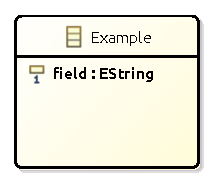
\includegraphics{images/05_library_of_transformations/02_type_level_transformations/06_data_fields/data_field.pdf}
        \caption{$Tm_{DataField}$ for a $\type{string}$ with $name = \type{field}$}
        \label{fig:library_of_transformations:type_level_transformations:data_fields:visualisation:ecore}
    \end{subfigure}
    \begin{subfigure}{0.45\textwidth}
        \centering
        % To use this figure in your LaTeX document
% import the package groove/resources/groove2tikz.sty
%
\begin{tikzpicture}[scale=\tikzscale,name prefix=test-]
\node[type_node] (n0) at (0.955, -0.775) {\ml{\textbf{Example}\\field: \textbf{string}}};

\end{tikzpicture}

        \caption{$TG_{DataField}$ for a $\type{string}$ with $name = \type{field}$}
        \label{fig:library_of_transformations:type_level_transformations:data_fields:visualisation:groove}
    \end{subfigure}
    \caption{Visualisation of the transformation of a field typed by a data type}
    \label{fig:library_of_transformations:type_level_transformations:data_fields:visualisation}
\end{figure}

All transformations discussed so far have focused on introducing different kind of types. In the following transformations, these types will be enriched with fields. In this transformation specifically, a field typed by a data type will be introduced.

\begin{defin}[Type model $Tm_{DataField}$]
\label{defin:library_of_transformations:type_level_transformations:data_fields:tmod_data_field}
Let $Tm_{DataField}$ be the type model containing a regular class with identifier $classtype$. Then $Tm_{DataField}$ defines a field named $name$ with type $fieldtype$, in which $fieldtype$ is either $\type{boolean}$, $\type{integer}$, $\type{real}$ or $\type{string}$. $Tm_{DataField}$ is defined as:
\begin{align*}
Class =\ &\{classtype\} \\
Enum =\ &\{\} \\
UserDataType =\ &\{\} \\
Field =\ &\{(classtype, name)\} \\
\mathrm{FieldSig} =\ &\begin{cases}
    (f, (fieldtype, 1..1)) &\mathrm{if}\ f \in Field_{Tm_{DataField}}
\end{cases} \\
EnumValue =\ &\{\} \\
Inh =\ &\{\} \\
Prop =\ &\{\} \\
Constant =\ &\{\} \\
\mathrm{ConstType} =\ &\{\}
\end{align*}
\isabellelref{tmod_data_field}{Ecore-GROOVE-Mapping-Library.DataField}
\end{defin}

\begin{thm}[Correctness of $Tm_{DataField}$]
\label{defin:library_of_transformations:type_level_transformations:data_fields:tmod_data_field_correct}
$Tm_{DataField}$ (\cref{defin:library_of_transformations:type_level_transformations:data_fields:tmod_data_field}) is a consistent type model in the sense of \cref{defin:formalisations:ecore_formalisation:type_models:type_model_consistency}.
\isabellelref{tmod_data_field_correct}{Ecore-GROOVE-Mapping-Library.DataField}
\end{thm}

A visual representation of $Tm_{DataField}$ with field name $\type{field}$ on class $.\type{Example}$ can be seen in \cref{fig:library_of_transformations:type_level_transformations:data_fields:visualisation:ecore}. In this example, the $\type{string}$ type is chosen for the fieldtype, but any data type would have worked. The correctness proof of $Tm_{DataField}$ is more involved, it is not included here for conciseness. It can be found within the validated Isabelle proofs.

In order to make composing transformation functions possible, $Tm_{DataField}$ should be compatible with the type model it is combined with.

\begin{thm}[Correctness of $\mathrm{combine}(Tm, Tm_{DataField})$]
\label{defin:library_of_transformations:type_level_transformations:data_fields:tmod_data_field_combine_correct}
Assume a type model $Tm$ that is consistent in the sense of \cref{defin:formalisations:ecore_formalisation:type_models:type_model_consistency}. Then $Tm$ is compatible with $Tm_{DataField}$ (in the sense of \cref{defin:transformation_framework:type_models_and_type_graphs:combining_type_models:compatibility}) if:
\begin{itemize}
    \item The class type on which the field is defined, $classtype$, is already an existing class in $Tm$;
    \item The field named $name$ is not already a field on $classtype$ in $Tm$.
\end{itemize}
\isabellelref{tmod_data_field_combine_correct}{Ecore-GROOVE-Mapping-Library.DataField}
\end{thm}

\begin{proof}
Use \cref{defin:transformation_framework:type_models_and_type_graphs:combining_type_models:tmod_combine_merge_correct}. It is possible to show that all assumptions hold. Now we have shown that $\mathrm{combine}(Tm, Tm_{DataField})$ is consistent in the sense of \cref{defin:formalisations:ecore_formalisation:type_models:type_model_consistency}.
\end{proof}

The definitions and theorems for defining a data field within Ecore are now complete. 

\subsubsection{Encoding as edge type}

The most obvious encoding for an field in GROOVE would be using an edge type. The field is transformed into an edge type between an existing node type and the corresponding field type. The encoding corresponding to $Tm_{DataField}$ can then be represented as $TG_{DataField}$, defined in the following definition:

\begin{defin}[Type graph $TG_{DataField}$]
\label{defin:library_of_transformations:type_level_transformations:data_fields:tg_data_field_as_edge_type}
Let $TG_{DataField}$ be the type graph containing a node type which encodes the class type $classtype$. Furthermore, define an edge type from $classtype$ named $name$. This edge type targets a node of $fieldtype$. $TG_{DataField}$ is defined as:
\begin{align*}
NT =\ &\{\mathrm{ns\_\!to\_\!list}(classtype), fieldtype\} \\
ET =\ &\{(\mathrm{ns\_\!to\_\!list}(classtype), \langle name \rangle, fieldtype)\} \\
\!\!\sqsubseteq\ =\ &\{( \mathrm{ns\_\!to\_\!list}(classtype), \mathrm{ns\_\!to\_\!list}(classtype) ), ( fieldtype, fieldtype )\} \\
abs =\ &\{\} \\
\mathrm{mult}(e) =\ &\begin{cases}
    (0..\mstar, 1..1) &\mathrm{if}\ e \in \{(\mathrm{ns\_\!to\_\!list}(classtype), \langle name \rangle, fieldtype)\}
\end{cases} \\
contains =\ &\{\}
\end{align*}
\isabellelref{tg_data_field_as_edge_type}{Ecore-GROOVE-Mapping-Library.DataField}
\end{defin}

\begin{thm}[Correctness of $TG_{DataField}$]
\label{defin:library_of_transformations:type_level_transformations:data_fields:tg_data_field_as_edge_type_correct}
$TG_{DataField}$ (\cref{defin:library_of_transformations:type_level_transformations:data_fields:tg_data_field_as_edge_type}) is a valid type graph in the sense of \cref{defin:formalisations:groove_formalisation:type_graphs:type_graph_validity}.
\isabellelref{tg_data_field_as_edge_type_correct}{Ecore-GROOVE-Mapping-Library.DataField}
\end{thm}

A visual representation of $TG_{DataField}$ with edge name $\type{field}$ on node type $\type{Example}$ can be seen in \cref{fig:library_of_transformations:type_level_transformations:data_fields:visualisation:groove}. Like the previous example, a $\type{string}$ has been chosen to be consequent, but any primitive type could have been used. The correctness proof of $TG_{DataField}$ is more involved, it is not included here for conciseness. It can be found within the validated Isabelle proofs.

In order to make composing transformation functions possible, $TG_{DataField}$ should be compatible with the type graph it is combined with.

\begin{thm}[Correctness of $\mathrm{combine}(TG, TG_{DataField})$]
\label{defin:library_of_transformations:type_level_transformations:data_fields:tg_data_field_as_edge_type_combine_correct}
Assume a type graph $TG$ that is valid in the sense of \cref{defin:formalisations:groove_formalisation:type_graphs:type_graph_validity}. Then $TG$ is compatible with $TG_{DataField}$ (in the sense of \cref{defin:transformation_framework:type_models_and_type_graphs:combining_type_graphs:compatibility}) if:
\begin{itemize}
    \item The node type of the encoded class type in $TG_{DataField}$ is already an node type in $TG$;
    \item The node type of the encoded class type in $TG_{DataField}$ does not already have an edge type with the same name as the field in $TG$.
\end{itemize}
\isabellelref{tg_data_field_as_edge_type_combine_correct}{Ecore-GROOVE-Mapping-Library.DataField}
\end{thm}

\begin{proof}
Use \cref{defin:transformation_framework:type_models_and_type_graphs:combining_type_graphs:tg_combine_merge_correct}. It is possible to show that all assumptions hold. Now we have shown that $\mathrm{combine}(TG, TG_{DataField})$ is valid in the sense of \cref{defin:formalisations:groove_formalisation:type_graphs:type_graph_validity}.
\end{proof}

The next definitions define the transformation function from $Tm_{DataField}$ to $TG_{DataField}$:

\begin{defin}[Transformation function $f_{DataField}$]
\label{defin:library_of_transformations:type_level_transformations:data_fields:tmod_data_field_to_tg_data_field_as_edge_type}
The transformation function $f_{DataField}(Tm)$ is defined as:
\begin{align*}
NT =\ &\{\mathrm{ns\_\!to\_\!list}(c) \mid c \in Class_{Tm}\} \cup \{fieldtype\}\\
ET =\ &\{(\mathrm{ns\_\!to\_\!list}(c), \langle f \rangle, fieldtype) \mid (c, n) \in Field_{Tm} \} \\
\!\!\sqsubseteq\ =\ &\{( \mathrm{ns\_\!to\_\!list}(c), \mathrm{ns\_\!to\_\!list}(c) ) \mid c \in Class_{Tm} \} \cup \{( fieldtype, fieldtype ) \} \\
abs =\ &\{\} \\
\mathrm{mult} =\ &\begin{cases}
    (0..\mstar, 1..1) &\mathrm{if}\ e \in \{(\mathrm{ns\_\!to\_\!list}(c), \langle f \rangle, fieldtype) \mid (c, n) \in Field_{Tm} \}
\end{cases} \\
contains =\ &\{\}
\end{align*}
\isabellelref{tmod_data_field_to_tg_data_field_as_edge_type}{Ecore-GROOVE-Mapping-Library.DataField}
\end{defin}

\begin{thm}[Correctness of $f_{DataField}$]
\label{defin:library_of_transformations:type_level_transformations:data_fields:tmod_data_field_to_tg_data_field_as_edge_type_func}
$f_{DataField}(Tm)$ (\cref{defin:library_of_transformations:type_level_transformations:data_fields:tmod_data_field_to_tg_data_field_as_edge_type}) is a valid transformation function in the sense of \cref{defin:transformation_framework:type_models_and_type_graphs:combining_transformation_functions:transformation_function_type_model_type_graph} transforming $Tm_{DataField}$ into $TG_{DataField}$.
\isabellelref{tmod_data_field_to_tg_data_field_as_edge_type_func}{Ecore-GROOVE-Mapping-Library.DataField}
\end{thm}

The proof of the correctness of $f_{DataField}$ will not be included here. Instead, it can be found in the validated Isabelle theories.

Finally, to complete the transformation, the transformation function that transforms $TG_{DataField}$ into $Tm_{DataField}$ is defined:

\begin{defin}[Transformation function $f'_{DataField}$]
\label{defin:library_of_transformations:type_level_transformations:data_fields:tg_data_field_as_edge_type_to_tmod_data_field}
The transformation function $f'_{DataField}(TG)$ is defined as:
\begin{align*}
Class =\ &\{\mathrm{list\_\!to\_\!ns}(n) \mid n \in NT_{TG} \cap Lab_t \} \\
Enum =\ &\{\} \\
UserDataType =\ &\{\} \\
Field =\ &\{(\mathrm{list\_\!to\_\!ns}(\mathrm{src}(e)), l) \mid e \in ET_{TG} \land \langle l \rangle = \mathrm{lab}(e) \} \\
\mathrm{FieldSig} =\ &\begin{cases}
    (f, (fieldtype, 1..1)) &\mathrm{if}\ f \in \{(\mathrm{list\_\!to\_\!ns}(\mathrm{src}(e)), l) \mid e \in ET_{TG} \land \langle l \rangle = \mathrm{lab}(e) \} 
\end{cases} \\
EnumValue =\ &\{\} \\
Inh =\ &\{\} \\
Prop =\ &\{\} \\
Constant =\ &\{\} \\
\mathrm{ConstType} =\ &\{\}
\end{align*}
\isabellelref{tg_data_field_as_edge_type_to_tmod_data_field}{Ecore-GROOVE-Mapping-Library.DataField}
\end{defin}

\begin{thm}[Correctness of $f'_{DataField}$]
\label{defin:library_of_transformations:type_level_transformations:data_fields:tg_data_field_as_edge_type_to_tmod_data_field_func}
$f'_{DataField}(TG)$ (\cref{defin:library_of_transformations:type_level_transformations:data_fields:tg_data_field_as_edge_type_to_tmod_data_field}) is a valid transformation function in the sense of \cref{defin:transformation_framework:type_models_and_type_graphs:combining_transformation_functions:transformation_function_type_graph_type_model} transforming $TG_{DataField}$ into $Tm_{DataField}$.
\isabellelref{tg_data_field_as_edge_type_to_tmod_data_field_func}{Ecore-GROOVE-Mapping-Library.DataField}
\end{thm}

Once more, the correctness proof is not included here but can be found in the validated Isabelle proofs of this thesis.
\subsection{Enumeration fields}
\label{subsec:library_of_transformations:type_level_transformations:enum_fields}

\begin{figure}
    \centering
    \begin{subfigure}{0.45\textwidth}
        \centering
        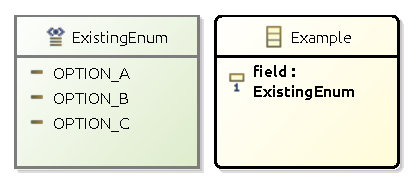
\includegraphics{images/05_library_of_transformations/02_type_level_transformations/07_enum_fields/enum_field.pdf}
        \caption{$Tm_{EnumField}$ for $.\type{ExistingEnum}$ \\with $name = \type{field}$}
        \label{fig:library_of_transformations:type_level_transformations:enum_fields:visualisation:ecore}
    \end{subfigure}
    \begin{subfigure}{0.45\textwidth}
        \centering
        % To use this figure in your LaTeX document
% import the package groove/resources/groove2tikz.sty
%
\begin{tikzpicture}[scale=\tikzscale,name prefix=test-]
\node[type_node] (n0) at (3.125, -0.945) {\ml{\textbf{Example}}};
\node[type_node] (n2) at (5.570, -0.970) {\ml{\textbf{ExistingEnum}\\\textit{OPTION\_A}\\\textit{OPTION\_B}\\\textit{OPTION\_C}}};

\path[basic_edge](n0.east |- 5.570, -0.970) -- node[lab] {\ml{field}} (n2) ;
\end{tikzpicture}

        \caption{$TG_{EnumFieldFlags}$ for $\type{ExistingEnum}$ \\with $name = \type{field}$}
        \label{fig:library_of_transformations:type_level_transformations:enum_fields:visualisation:groove_flags}
    \end{subfigure}
    \\
    \begin{subfigure}{0.95\textwidth}
        \centering
        % To use this figure in your LaTeX document
% import the package groove/resources/groove2tikz.sty
%
\begin{tikzpicture}[scale=\tikzscale,name prefix=test-]
\node[type_node] (n0) at (3.125, -0.945) {\ml{\textbf{Example}}};
\node[type_node] (n2) at (5.570, -0.970) {\ml{\textit{\textbf{ExistingEnum}}}};
\node[type_node] (n3) at (2.970, -0.170) {\ml{\textbf{ExistingEnum\$OPTION\_A}}};
\node[type_node] (n4) at (5.570, -0.170) {\ml{\textbf{ExistingEnum\$OPTION\_B}}};
\node[type_node] (n5) at (8.170, -0.170) {\ml{\textbf{ExistingEnum\$OPTION\_C}}};

\path[subtype_edge] (n3)  --  (n2) ;
\path[subtype_edge](n4.south -| 5.570, -0.970) --  (n2) ;
\path[subtype_edge] (n5)  --  (n2) ;
\path[basic_edge](n0.east |- 5.570, -0.970) -- node[lab] {\ml{field}} (n2) ;
\end{tikzpicture}

        \caption{$TG_{EnumFieldNodes}$ for $\type{ExistingEnum}$ with $name = \type{field}$}
        \label{fig:library_of_transformations:type_level_transformations:enum_fields:visualisation:groove_nodes}
    \end{subfigure}
    \caption{Visualisation of the transformation of a field typed by an enumeration type}
    \label{fig:library_of_transformations:type_level_transformations:enum_fields:visualisation}
\end{figure}

In this section, the transformation for a field typed by an enumeration type will be discussed. Since an enumeration type can be encoded in multiple ways, multiple encodings will be introduced for fields as well. First, the Ecore type model will be introduced.

\begin{defin}[Type model $Tm_{EnumField}$]
\label{defin:library_of_transformations:type_level_transformations:enum_fields:tmod_enum_field}
Let $Tm_{EnumField}$ be the type model containing a regular class with identifier $classtype$. Furthermore, it defines an enumeration type with identifier $enumid$, and corresponding values as set $enumvalues$. Then $Tm_{EnumField}$ defines a field named $name$ with type $enumid$ on class $classtype$. $Tm_{EnumField}$ is defined as:
\begin{align*}
Class =\ &\{classtype\} \\
Enum =\ &\{enumid\} \\
UserDataType =\ &\{\} \\
Field =\ &\{(classtype, name)\} \\
\mathrm{FieldSig} =\ &\begin{cases}
    (f, (enumid, 1..1)) &\mathrm{if}\ f \in Field_{Tm_{EnumField}}
\end{cases} \\
EnumValue =\ &\{(enumid, v) \mid v \in enumvalues\} \\
Inh =\ &\{\} \\
Prop =\ &\{\} \\
Constant =\ &\{\} \\
\mathrm{ConstType} =\ &\{\}
\end{align*}
\isabellelref{tmod_enum_field}{Ecore-GROOVE-Mapping-Library.EnumField}
\end{defin}

\begin{thm}[Correctness of $Tm_{EnumField}$]
\label{defin:library_of_transformations:type_level_transformations:enum_fields:tmod_enum_field_correct}
$Tm_{EnumField}$ (\cref{defin:library_of_transformations:type_level_transformations:enum_fields:tmod_enum_field}) is a consistent type model in the sense of \cref{defin:formalisations:ecore_formalisation:type_models:type_model_consistency}.
\isabellelref{tmod_enum_field_correct}{Ecore-GROOVE-Mapping-Library.EnumField}
\end{thm}

A visual representation of $Tm_{EnumField}$ with field name $\type{field}$ on class $.\type{Example}$ can be seen in \cref{fig:library_of_transformations:type_level_transformations:enum_fields:visualisation:ecore}. In this example, the field is typed by the $.\type{ExistingEnum}$ enumeration type. The correctness proof of $Tm_{EnumField}$ is more involved, it is not included here for conciseness. It can be found within the validated Isabelle proofs.

In order to make composing transformation functions possible, $Tm_{EnumField}$ should be compatible with the type model it is combined with.

\begin{thm}[Correctness of $\mathrm{combine}(Tm, Tm_{EnumField})$]
\label{defin:library_of_transformations:type_level_transformations:enum_fields:tmod_enum_field_combine_correct}
Assume a type model $Tm$ that is consistent in the sense of \cref{defin:formalisations:ecore_formalisation:type_models:type_model_consistency}. Then $Tm$ is compatible with $Tm_{EnumField}$ (in the sense of \cref{defin:transformation_framework:type_models_and_type_graphs:combining_type_models:compatibility}) if:
\begin{itemize}
    \item The class type on which the field is defined, $classtype$, is already an existing class in $Tm$;
    \item The enumeration type by which the field is typed, $enumid$, is already an existing enumeration type in $Tm$;
    \item All the values for the enumeration type $enumid$ are already enumeration values for $enumid$ in $Tm$;
    \item The field named $name$ is not already a field on $classtype$ in $Tm$.
\end{itemize}
\isabellelref{tmod_enum_field_combine_correct}{Ecore-GROOVE-Mapping-Library.EnumField}
\end{thm}

\begin{proof}
Use \cref{defin:transformation_framework:type_models_and_type_graphs:combining_type_models:tmod_combine_merge_correct}. It is possible to show that all assumptions hold. Now we have shown that $\mathrm{combine}(Tm, Tm_{EnumField})$ is consistent in the sense of \cref{defin:formalisations:ecore_formalisation:type_models:type_model_consistency}.
\end{proof}

The definitions and theorems for defining a field typed by an enumeration type within Ecore are now complete. 

\subsubsection{Encoding as edge type to an node type encoded enumeration type}

As mentioned earlier, \cref{subsec:library_of_transformations:type_level_transformations:enumeration_types} defines multiple ways to encode an enumeration type. Each of these encodings needs a specialised field encoding. In principle, the encoding of the fields itself is the same, but since every transformation model needs to be valid on its own, the encodings need to be distinguished. 

The first encoding for an enumeration type uses node types to encode the different values. The encoding corresponding to $Tm_{EnumField}$, in the case that the field references an enumeration type encoded as node types, can then be represented as $TG_{EnumFieldNodes}$, defined in the following definition:

\begin{defin}[Type graph $TG_{EnumFieldNodes}$]
\label{defin:library_of_transformations:type_level_transformations:enum_fields:tg_enum_as_node_types_field_as_edge_type}
Let $TG_{EnumFieldNodes}$ be the type graph containing a node type which encodes the class type $classtype$.
Furthermore, $TG_{EnumFieldNodes}$ contains an encoded version of enumeration type $enumid$ with values from set $enumvalues$. This enumeration type is encoded using node types, as defined in $TG_{EnumNodes}$ (\cref{defin:library_of_transformations:type_level_transformations:enumeration_types:tg_enum_as_node_types}). Finally, $TG_{EnumFieldNodes}$ defines an edge type from the encoded $classtype$ named $name$ to the encoded enumeration type $enumid$. $TG_{EnumFieldNodes}$ is defined as:
\begin{align*}
NT =\ &\{\mathrm{ns\_\!to\_\!list}(classtype), \mathrm{ns\_\!to\_\!list}(enumid)\}\ \cup \\&\{ \mathrm{ns\_\!to\_\!list}(enumid) \append \langle v \rangle \mid v \in enumvalues \}\\
ET =\ &\{(\mathrm{ns\_\!to\_\!list}(classtype), \langle name \rangle, \mathrm{ns\_\!to\_\!list}(enumid))\} \\
\!\!\sqsubseteq\ =\ &\{(\mathrm{ns\_\!to\_\!list}(classtype), \mathrm{ns\_\!to\_\!list}(classtype)),\ \\& (\mathrm{ns\_\!to\_\!list}(enumid), \mathrm{ns\_\!to\_\!list}(enumid))\}\ \cup \\&
\{(\mathrm{ns\_\!to\_\!list}(enumid) \append \langle v \rangle, \mathrm{ns\_\!to\_\!list}(enumid) \append \langle v \rangle) \mid v \in enumvalues \}\ \cup \\&
\{(\mathrm{ns\_\!to\_\!list}(enumid) \append \langle v \rangle, \mathrm{ns\_\!to\_\!list}(enumid)) \mid v \in enumvalues \} \\
abs =\ &\{\mathrm{ns\_\!to\_\!list}(enumid)\} \\
\mathrm{mult}(e) =\ &\begin{cases}
    (0..\mstar, 1..1) &\mathrm{if}\ e \in \{(\mathrm{ns\_\!to\_\!list}(classtype), \langle name \rangle, \mathrm{ns\_\!to\_\!list}(enumid))\}
\end{cases} \\
contains =\ &\{\}
\end{align*}
\isabellelref{tg_enum_as_node_types_field_as_edge_type}{Ecore-GROOVE-Mapping-Library.EnumField}
\end{defin}

\begin{thm}[Correctness of $TG_{EnumFieldNodes}$]
\label{defin:library_of_transformations:type_level_transformations:enum_fields:tg_enum_as_node_types_field_as_edge_type_correct}
$TG_{EnumFieldNodes}$ (\cref{defin:library_of_transformations:type_level_transformations:enum_fields:tg_enum_as_node_types_field_as_edge_type}) is a valid type graph in the sense of \cref{defin:formalisations:groove_formalisation:type_graphs:type_graph_validity}.
\isabellelref{tg_enum_as_node_types_field_as_edge_type_correct}{Ecore-GROOVE-Mapping-Library.EnumField}
\end{thm}

A visual representation of $TG_{EnumFieldNodes}$ with edge name $\type{field}$ on node type $\type{Example}$ can be seen in \cref{fig:library_of_transformations:type_level_transformations:enum_fields:visualisation:groove_nodes}. The field references the encoded enumeration type $\type{ExistingEnum}$ via the abstract type, such that its nodes can reference any of the concrete values. The correctness proof of $TG_{EnumFieldNodes}$ is more involved, it is not included here for conciseness. It can be found within the validated Isabelle proofs.

In order to make composing transformation functions possible, $TG_{EnumFieldNodes}$ should be compatible with the type graph it is combined with.

\begin{thm}[Correctness of $\mathrm{combine}(TG, TG_{EnumFieldNodes})$]
\label{defin:library_of_transformations:type_level_transformations:enum_fields:tg_enum_as_node_types_field_as_edge_type_combine_correct}
Assume a type graph $TG$ that is valid in the sense of \cref{defin:formalisations:groove_formalisation:type_graphs:type_graph_validity}. Then $TG$ is compatible with $TG_{EnumFieldNodes}$ (in the sense of \cref{defin:transformation_framework:type_models_and_type_graphs:combining_type_graphs:compatibility}) if:
\begin{itemize}
    \item The node type of the encoded class type in $TG_{EnumFieldNodes}$ is already an node type in $TG$;
    \item All node types corresponding to the encoding of the enumeration type in $TG_{EnumFieldNodes}$ are already node types in $TG$;
    \item The node type of the encoded class type in $TG_{EnumFieldNodes}$ does not already have an edge type with the same name as the field in $TG$.
\end{itemize}
\isabellelref{tg_enum_as_node_types_field_as_edge_type_combine_correct}{Ecore-GROOVE-Mapping-Library.EnumField}
\end{thm}

\begin{proof}
Use \cref{defin:transformation_framework:type_models_and_type_graphs:combining_type_graphs:tg_combine_merge_correct}. It is possible to show that all assumptions hold. Now we have shown that $\mathrm{combine}(TG, TG_{EnumFieldNodes})$ is valid in the sense of \cref{defin:formalisations:groove_formalisation:type_graphs:type_graph_validity}.
\end{proof}

The next definitions define the transformation function from $Tm_{EnumField}$ to $TG_{EnumFieldNodes}$:

\begin{defin}[Transformation function $f_{EnumFieldNodes}$]
\label{defin:library_of_transformations:type_level_transformations:enum_fields:tmod_enum_field_to_tg_enum_as_node_types_field_as_edge_type}
The transformation function $f_{EnumFieldNodes}(Tm)$ is defined as:
\begin{align*}
NT =\ &\{\mathrm{ns\_\!to\_\!list}(t) \mid t \in Class_{Tm} \cup Enum_{Tm}\}\ \cup \\&\{ \mathrm{ns\_\!to\_\!list}(e) \append \langle v \rangle \mid (e, v) \in EnumValue_{Tm} \}\\
ET =\ &\{(\mathrm{ns\_\!to\_\!list}(c), \langle f \rangle, \mathrm{ns\_\!to\_\!list}(e)) \mid (c, f) \in Field_{Tm} \land e \in Enum_{Tm}\} \\
\!\!\sqsubseteq\ =\ &\{(\mathrm{ns\_\!to\_\!list}(x), \mathrm{ns\_\!to\_\!list}(x)) \mid x \in Class_{Tm} \cup Enum_{Tm} \}\ \cup \\&
\{(\mathrm{ns\_\!to\_\!list}(e) \append \langle v \rangle, \mathrm{ns\_\!to\_\!list}(e) \append \langle v \rangle) \mid (e, v) \in EnumValue_{Tm} \}\ \cup \\&
\{(\mathrm{ns\_\!to\_\!list}(e) \append \langle v \rangle, \mathrm{ns\_\!to\_\!list}(e)) \mid (e, v) \in EnumValue_{Tm} \} \\
abs =\ &\{\mathrm{ns\_\!to\_\!list}(t) \mid t \in Enum_{Tm}\}\ \\
\mathrm{mult}(e) =\ &\begin{cases}
    (0..\mstar, 1..1) &\mathrm{if}\ e \in \{(\mathrm{ns\_\!to\_\!list}(c), \langle f \rangle, \mathrm{ns\_\!to\_\!list}(e)) \mid (c, f) \in Field_{Tm} \land e \in Enum_{Tm}\}
\end{cases} \\
contains =\ &\{\}
\end{align*}
\isabellelref{tmod_enum_field_to_tg_enum_as_node_types_field_as_edge_type}{Ecore-GROOVE-Mapping-Library.EnumField}
\end{defin}

\begin{thm}[Correctness of $f_{EnumFieldNodes}$]
\label{defin:library_of_transformations:type_level_transformations:enum_fields:tmod_enum_field_to_tg_enum_as_node_types_field_as_edge_type_func}
$f_{EnumFieldNodes}(Tm)$ (\cref{defin:library_of_transformations:type_level_transformations:enum_fields:tmod_enum_field_to_tg_enum_as_node_types_field_as_edge_type}) is a valid transformation function in the sense of \cref{defin:transformation_framework:type_models_and_type_graphs:combining_transformation_functions:transformation_function_type_model_type_graph} transforming $Tm_{EnumField}$ into $TG_{EnumFieldNodes}$.
\isabellelref{tmod_enum_field_to_tg_enum_as_node_types_field_as_edge_type_func}{Ecore-GROOVE-Mapping-Library.EnumField}
\end{thm}

The proof of the correctness of $f_{EnumFieldNodes}$ will not be included here. Instead, it can be found in the validated Isabelle theories.

Finally, to complete the transformation, the transformation function that transforms $TG_{EnumFieldNodes}$ into $Tm_{EnumField}$ is defined:

\begin{defin}[Transformation function $f'_{EnumFieldNodes}$]
\label{defin:library_of_transformations:type_level_transformations:enum_fields:tg_enum_as_node_types_field_as_edge_type_to_tmod_enum_field}
The transformation function $f'_{EnumFieldNodes}(TG)$ is defined as:
\begin{align*}
Class =\ &\{\mathrm{list\_\!to\_\!ns}(n) \mid n \in NT_{TG} \land n = \mathrm{ns\_\!to\_\!list}(classtype) \} \\
Enum =\ &\{\mathrm{list\_\!to\_\!ns}(n) \mid n \in NT_{TG} \land n = \mathrm{ns\_\!to\_\!list}(enumid) \} \\
UserDataType =\ &\{\} \\
Field =\ &\{(\mathrm{list\_\!to\_\!ns}(\mathrm{src}(e)), l) \mid e \in ET_{TG} \land \langle l \rangle = \mathrm{lab}(e) \} \\
\mathrm{FieldSig} =\ &\begin{cases}
    (f, (fieldtype, 1..1)) &\mathrm{if}\ f \in \{(\mathrm{list\_\!to\_\!ns}(\mathrm{src}(e)), l) \mid e \in ET_{TG} \land \langle l \rangle = \mathrm{lab}(e) \}
\end{cases} \\
EnumValue =\ &\{(enumid, v) \mid v \in enumvalues\} \\
Inh =\ &\{\} \\
Prop =\ &\{\} \\
Constant =\ &\{\} \\
\mathrm{ConstType} =\ &\{\}
\end{align*}
\isabellelref{tg_enum_as_node_types_field_as_edge_type_to_tmod_enum_field}{Ecore-GROOVE-Mapping-Library.EnumField}
\end{defin}

\begin{thm}[Correctness of $f'_{EnumFieldNodes}$]
\label{defin:library_of_transformations:type_level_transformations:enum_fields:tg_enum_as_node_types_field_as_edge_type_to_tmod_enum_field_func}
$f'_{EnumFieldNodes}(TG)$ (\cref{defin:library_of_transformations:type_level_transformations:enum_fields:tg_enum_as_node_types_field_as_edge_type_to_tmod_enum_field}) is a valid transformation function in the sense of \cref{defin:transformation_framework:type_models_and_type_graphs:combining_transformation_functions:transformation_function_type_graph_type_model} transforming $TG_{EnumFieldNodes}$ into $Tm_{EnumField}$.
\isabellelref{tg_enum_as_node_types_field_as_edge_type_to_tmod_enum_field_func}{Ecore-GROOVE-Mapping-Library.EnumField}
\end{thm}

Once more, the correctness proof is not included here but can be found in the validated Isabelle proofs of this thesis.

\subsubsection{Encoding as edge type to an flag encoded enumeration type}

The second encoding for an enumeration type uses flags to encode the different values. The encoding corresponding to $Tm_{EnumField}$, in the case that the field references an enumeration type encoded as flags, can then be represented as $TG_{EnumFieldFlags}$, defined in the following definition:

\begin{defin}[Type graph $TG_{EnumFieldFlags}$]
\label{defin:library_of_transformations:type_level_transformations:enum_fields:tg_enum_as_flags_field_as_edge_type}
Let $TG_{EnumFieldFlags}$ be the type graph containing a node type which encodes the class type $classtype$.
Furthermore, $TG_{EnumFieldFlags}$ contains an encoded version of enumeration type $enumid$ with values from set $enumvalues$. This enumeration type is encoded using flags, as defined in $TG_{EnumFlags}$ (\cref{defin:library_of_transformations:type_level_transformations:enumeration_types:tg_enum_as_flags}). Finally, $TG_{EnumFieldFlags}$ defines an edge type from the encoded $classtype$ named $name$ to the encoded enumeration type $enumid$. $TG_{EnumFieldFlags}$ is defined as:
\begin{align*}
NT =\ &\{\mathrm{ns\_\!to\_\!list}(classtype), \mathrm{ns\_\!to\_\!list}(enumid)\}\\
ET =\ &\{(\mathrm{ns\_\!to\_\!list}(classtype), \langle name \rangle, \mathrm{ns\_\!to\_\!list}(enumid))\}\\
\!\!\sqsubseteq\ =\ &\{(\mathrm{ns\_\!to\_\!list}(classtype), \mathrm{ns\_\!to\_\!list}(classtype)),\ \\& (\mathrm{ns\_\!to\_\!list}(enumid), \mathrm{ns\_\!to\_\!list}(enumid))\}\\
abs =\ &\{\} \\
\mathrm{mult}(e) =\ &\begin{cases}
    (0..\mstar, 1..1) &\mathrm{if}\ e \in \{(\mathrm{ns\_\!to\_\!list}(classtype), \langle name \rangle, \mathrm{ns\_\!to\_\!list}(enumid))\}
\end{cases} \\
contains =\ &\{\}
\end{align*}
\isabellelref{tg_enum_as_flags_field_as_edge_type}{Ecore-GROOVE-Mapping-Library.EnumField}
\end{defin}

\begin{thm}[Correctness of $TG_{EnumFieldFlags}$]
\label{defin:library_of_transformations:type_level_transformations:enum_fields:tg_enum_as_flags_field_as_edge_type_correct}
$TG_{EnumFieldFlags}$ (\cref{defin:library_of_transformations:type_level_transformations:enum_fields:tg_enum_as_flags_field_as_edge_type}) is a valid type graph in the sense of \cref{defin:formalisations:groove_formalisation:type_graphs:type_graph_validity}.
\isabellelref{tg_enum_as_flags_field_as_edge_type_correct}{Ecore-GROOVE-Mapping-Library.EnumField}
\end{thm}

A visual representation of $TG_{EnumFieldFlags}$ with edge name $\type{field}$ on node type $\type{Example}$ can be seen in \cref{fig:library_of_transformations:type_level_transformations:enum_fields:visualisation:groove_flags}. The field references the encoded enumeration type $\type{ExistingEnum}$ via the corresponding node type. The correctness proof of $TG_{EnumFieldFlags}$ is more involved, it is not included here for conciseness. It can be found within the validated Isabelle proofs.

In order to make composing transformation functions possible, $TG_{EnumFieldFlags}$ should be compatible with the type graph it is combined with.

\begin{thm}[Correctness of $\mathrm{combine}(TG, TG_{EnumFieldFlags})$]
\label{defin:library_of_transformations:type_level_transformations:enum_fields:tg_enum_as_flags_field_as_edge_type_combine_correct}
Assume a type graph $TG$ that is valid in the sense of \cref{defin:formalisations:groove_formalisation:type_graphs:type_graph_validity}. Then $TG$ is compatible with $TG_{EnumFieldFlags}$ (in the sense of \cref{defin:transformation_framework:type_models_and_type_graphs:combining_type_graphs:compatibility}) if:
\begin{itemize}
    \item The node type of the encoded class type in $TG_{EnumFieldFlags}$ is already an node type in $TG$;
    \item All node types corresponding to the encoding of the enumeration type in $TG_{EnumFieldFlags}$ are already node types in $TG$;
    \item The node type of the encoded class type in $TG_{EnumFieldFlags}$ does not already have an edge type with the same name as the field in $TG$.
\end{itemize}
\isabellelref{tg_enum_as_flags_field_as_edge_type_combine_correct}{Ecore-GROOVE-Mapping-Library.EnumField}
\end{thm}

\begin{proof}
Use \cref{defin:transformation_framework:type_models_and_type_graphs:combining_type_graphs:tg_combine_merge_correct}. It is possible to show that all assumptions hold. Now we have shown that $\mathrm{combine}(TG, TG_{EnumFieldFlags})$ is valid in the sense of \cref{defin:formalisations:groove_formalisation:type_graphs:type_graph_validity}.
\end{proof}

The next definitions define the transformation function from $Tm_{EnumField}$ to $TG_{EnumFieldFlags}$:

\begin{defin}[Transformation function $f_{EnumFieldFlags}$]
\label{defin:library_of_transformations:type_level_transformations:enum_fields:tmod_enum_field_to_tg_enum_as_flags_field_as_edge_type}
The transformation function $f_{EnumFieldFlags}(Tm)$ is defined as:
\begin{align*}
NT =\ &\{\mathrm{ns\_\!to\_\!list}(t) \mid t \in Class_{Tm} \cup Enum_{Tm}\}\\
ET =\ &\{(\mathrm{ns\_\!to\_\!list}(c), \langle f \rangle, \mathrm{ns\_\!to\_\!list}(e)) \mid (c, f) \in Field_{Tm} \land e \in Enum_{Tm}\} \\
\!\!\sqsubseteq\ =\ &\{(\mathrm{ns\_\!to\_\!list}(x), \mathrm{ns\_\!to\_\!list}(x)) \mid x \in Class_{Tm} \cup Enum_{Tm} \}\\
abs =\ &\{\}\ \\
\mathrm{mult}(e) =\ &\begin{cases}
    (0..\mstar, 1..1) &\mathrm{if}\ e \in \{(\mathrm{ns\_\!to\_\!list}(c), \langle f \rangle, \mathrm{ns\_\!to\_\!list}(e)) \mid (c, f) \in Field_{Tm} \land e \in Enum_{Tm}\}
\end{cases} \\
contains =\ &\{\}
\end{align*}
\isabellelref{tmod_enum_field_to_tg_enum_as_flags_field_as_edge_type}{Ecore-GROOVE-Mapping-Library.EnumField}
\end{defin}

\begin{thm}[Correctness of $f_{EnumFieldFlags}$]
\label{defin:library_of_transformations:type_level_transformations:enum_fields:tmod_enum_field_to_tg_enum_as_flags_field_as_edge_type_func}
$f_{EnumFieldFlags}(Tm)$ (\cref{defin:library_of_transformations:type_level_transformations:enum_fields:tmod_enum_field_to_tg_enum_as_flags_field_as_edge_type}) is a valid transformation function in the sense of \cref{defin:transformation_framework:type_models_and_type_graphs:combining_transformation_functions:transformation_function_type_model_type_graph} transforming $Tm_{EnumField}$ into $TG_{EnumFieldFlags}$.
\isabellelref{tmod_enum_field_to_tg_enum_as_flags_field_as_edge_type_func}{Ecore-GROOVE-Mapping-Library.EnumField}
\end{thm}

The proof of the correctness of $f_{EnumFieldFlags}$ will not be included here. Instead, it can be found in the validated Isabelle theories.

Finally, to complete the transformation, the transformation function that transforms $TG_{EnumFieldFlags}$ into $Tm_{EnumField}$ is defined:

\begin{defin}[Transformation function $f'_{EnumFieldFlags}$]
\label{defin:library_of_transformations:type_level_transformations:enum_fields:tg_enum_as_flags_field_as_edge_type_to_tmod_enum_field}
The transformation function $f'_{EnumFieldFlags}(TG)$ is defined as:
\begin{align*}
Class =\ &\{\mathrm{list\_\!to\_\!ns}(n) \mid n \in NT_{TG} \land n = \mathrm{ns\_\!to\_\!list}(classtype) \} \\
Enum =\ &\{\mathrm{list\_\!to\_\!ns}(n) \mid n \in NT_{TG} \land n = \mathrm{ns\_\!to\_\!list}(enumid) \} \\
UserDataType =\ &\{\} \\
Field =\ &\{(\mathrm{list\_\!to\_\!ns}(\mathrm{src}(e)), l) \mid e \in ET_{TG} \land \langle l \rangle = \mathrm{lab}(e) \} \\
\mathrm{FieldSig} =\ &\begin{cases}
    (f, (fieldtype, 1..1)) &\mathrm{if}\ f \in \{(\mathrm{list\_\!to\_\!ns}(\mathrm{src}(e)), l) \mid e \in ET_{TG} \land \langle l \rangle = \mathrm{lab}(e) \}
\end{cases} \\
EnumValue =\ &\{(enumid, v) \mid v \in enumvalues\} \\
Inh =\ &\{\} \\
Prop =\ &\{\} \\
Constant =\ &\{\} \\
\mathrm{ConstType} =\ &\{\}
\end{align*}
\isabellelref{tg_enum_as_flags_field_as_edge_type_to_tmod_enum_field}{Ecore-GROOVE-Mapping-Library.EnumField}
\end{defin}

\begin{thm}[Correctness of $f'_{EnumFieldFlags}$]
\label{defin:library_of_transformations:type_level_transformations:enum_fields:tg_enum_as_flags_field_as_edge_type_to_tmod_enum_field_func}
$f'_{EnumFieldFlags}(TG)$ (\cref{defin:library_of_transformations:type_level_transformations:enum_fields:tg_enum_as_flags_field_as_edge_type_to_tmod_enum_field}) is a valid transformation function in the sense of \cref{defin:transformation_framework:type_models_and_type_graphs:combining_transformation_functions:transformation_function_type_graph_type_model} transforming $TG_{EnumFieldFlags}$ into $Tm_{EnumField}$.
\isabellelref{tg_enum_as_flags_field_as_edge_type_to_tmod_enum_field_func}{Ecore-GROOVE-Mapping-Library.EnumField}
\end{thm}

Once more, the correctness proof is not included here but can be found in the validated Isabelle proofs of this thesis.
\subsection{Nullable class fields}
\label{subsec:library_of_transformations:type_level_transformations:nullable_class_fields}

\begin{figure}
    \centering
    \begin{subfigure}{0.95\textwidth}
        \centering
        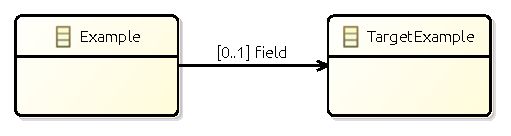
\includegraphics{images/05_library_of_transformations/02_type_level_transformations/08_nullable_class_fields/nullable_class_field.pdf}
        \caption{$Tm_{NullableClassField}$ to a class type $.\type{TargetExample}$ with $name = \type{field}$}
        \label{fig:library_of_transformations:type_level_transformations:nullable_class_fields:visualisation:ecore}
    \end{subfigure}
    \\
    \begin{subfigure}{0.95\textwidth}
        \centering
        % To use this figure in your LaTeX document
% import the package groove/resources/groove2tikz.sty
%
\begin{tikzpicture}[scale=\tikzscale,name prefix=test-]
\node[type_node] (n0) at (3.125, -0.945) {\ml{\textbf{Example}}};
\node[type_node] (n1) at (5.040, -0.950) {\ml{\textbf{TargetExample}}};

\path[basic_edge](n0.east |- 5.040, -0.950) -- node[lab] {\ml{field}} (n1) ;
\end{tikzpicture}

        \caption{$TG_{NullableClassField}$ to a class type $\type{TargetExample}$ with $name = \type{field}$}
        \label{fig:library_of_transformations:type_level_transformations:nullable_class_fields:visualisation:groove}
    \end{subfigure}
    \caption{Visualisation of the transformation of a field typed by an optional class type}
    \label{fig:library_of_transformations:type_level_transformations:nullable_class_fields:visualisation}
\end{figure}

The previous sections have shown transformations of fields to attribute types. It has not shown any relations between objects yet. This transformation defines the transformation of a nullable class field.

\begin{defin}[Type model $Tm_{NullableClassField}$]
\label{defin:library_of_transformations:type_level_transformations:nullable_class_fields:tmod_nullable_class_field}
Let $Tm_{NullableClassField}$ be the type model containing a regular class with identifier $classtype$. Then $Tm_{NullableClassField}$ defines a field named $name$ with type $fieldtype$, in which $fieldtype$ is the identifier of another class type in $Tm_{NullableClassField}$. $Tm_{NullableClassField}$ is defined as:
\begin{align*}
Class =\ &\{classtype, fieldtype\} \\
Enum =\ &\{\} \\
UserDataType =\ &\{\} \\
Field =\ &\{(classtype, name)\} \\
\mathrm{FieldSig} =\ &\begin{cases}
    (f, (?fieldtype, 0..1)) &\mathrm{if}\ f \in Field_{Tm_{NullableClassField}}
\end{cases} \\
EnumValue =\ &\{\} \\
Inh =\ &\{\} \\
Prop =\ &\{\} \\
Constant =\ &\{\} \\
\mathrm{ConstType} =\ &\{\}
\end{align*}
\isabellelref{tmod_nullable_class_field}{Ecore-GROOVE-Mapping-Library.NullableClassField}
\end{defin}

\begin{thm}[Correctness of $Tm_{NullableClassField}$]
\label{defin:library_of_transformations:type_level_transformations:nullable_class_fields:tmod_nullable_class_field_correct}
$Tm_{NullableClassField}$ (\cref{defin:library_of_transformations:type_level_transformations:nullable_class_fields:tmod_nullable_class_field}) is a consistent type model in the sense of \cref{defin:formalisations:ecore_formalisation:type_models:type_model_consistency}.
\isabellelref{tmod_nullable_class_field_correct}{Ecore-GROOVE-Mapping-Library.NullableClassField}
\end{thm}

A visual representation of $Tm_{NullableClassField}$ with field name $\type{field}$ on class $.\type{Example}$ can be seen in \cref{fig:library_of_transformations:type_level_transformations:nullable_class_fields:visualisation:ecore}. In this example, $\type{field}$ references a class of $.\type{TargetExample}$. Please note that the lower bound of the multiplicity is 0 as the class is considered nullable. That means that setting a value for $\type{field}$ on class $.\type{Example}$ is optional. The correctness proof of $Tm_{NullableClassField}$ is more involved, it is not included here for conciseness. It can be found within the validated Isabelle proofs.

In order to make composing transformation functions possible, $Tm_{NullableClassField}$ should be compatible with the type model it is combined with.

\begin{thm}[Correctness of $\mathrm{combine}(Tm, Tm_{NullableClassField})$]
\label{defin:library_of_transformations:type_level_transformations:nullable_class_fields:tmod_nullable_class_field_combine_correct}
Assume a type model $Tm$ that is consistent in the sense of \cref{defin:formalisations:ecore_formalisation:type_models:type_model_consistency}. Then $Tm$ is compatible with $Tm_{NullableClassField}$ (in the sense of \cref{defin:transformation_framework:type_models_and_type_graphs:combining_type_models:compatibility}) if:
\begin{itemize}
    \item The class type on which the field is defined, $classtype$, is already an existing class in $Tm$;
    \item The class type which the field targets, $fieldtype$, is already an existing class in $Tm$;
    \item The field named $name$ is not already a field on $classtype$ in $Tm$.
\end{itemize}
\isabellelref{tmod_nullable_class_field_combine_correct}{Ecore-GROOVE-Mapping-Library.NullableClassField}
\end{thm}

\begin{proof}
Use \cref{defin:transformation_framework:type_models_and_type_graphs:combining_type_models:tmod_combine_merge_correct}. It is possible to show that all assumptions hold. Now we have shown that $\mathrm{combine}(Tm, Tm_{NullableClassField})$ is consistent in the sense of \cref{defin:formalisations:ecore_formalisation:type_models:type_model_consistency}.
\end{proof}

The definitions and theorems for defining a data field within Ecore are now complete. 

\subsubsection{Encoding as edge type}

Like any field definition so far, an edge type will be used within GROOVE to encode the field. The field is transformed into an edge type from the encoded class type to the encoded target type. The encoding corresponding to $Tm_{NullableClassField}$ can then be represented as $TG_{NullableClassField}$, defined in the following definition:

\begin{defin}[Type graph $TG_{NullableClassField}$]
\label{defin:library_of_transformations:type_level_transformations:nullable_class_fields:tg_nullable_class_field_as_edge_type}
Let $TG_{NullableClassField}$ be the type graph containing a node type which encodes the class type $classtype$. Furthermore, define an edge type from $classtype$ named $name$. This edge type targets a node of $fieldtype$. $TG_{NullableClassField}$ is defined as:
\begin{align*}
NT =\ &\{\mathrm{ns\_\!to\_\!list}(classtype), \mathrm{ns\_\!to\_\!list}(fieldtype)\} \\
ET =\ &\{(\mathrm{ns\_\!to\_\!list}(classtype), \langle name \rangle, \mathrm{ns\_\!to\_\!list}(fieldtype))\} \\
\!\!\sqsubseteq\ =\ &\{( \mathrm{ns\_\!to\_\!list}(classtype), \mathrm{ns\_\!to\_\!list}(classtype) ),\\&( \mathrm{ns\_\!to\_\!list}(fieldtype), \mathrm{ns\_\!to\_\!list}(fieldtype) )\} \\
abs =\ &\{\} \\
\mathrm{mult}(e) =\ &\begin{cases}
    (0..\mstar, 0..1) &\mathrm{if}\ e \in \{(\mathrm{ns\_\!to\_\!list}(classtype), \langle name \rangle, \mathrm{ns\_\!to\_\!list}(fieldtype))\}
\end{cases} \\
contains =\ &\{\}
\end{align*}
\isabellelref{tg_nullable_class_field_as_edge_type}{Ecore-GROOVE-Mapping-Library.NullableClassField}
\end{defin}

\begin{thm}[Correctness of $TG_{NullableClassField}$]
\label{defin:library_of_transformations:type_level_transformations:nullable_class_fields:tg_nullable_class_field_as_edge_type_correct}
$TG_{NullableClassField}$ (\cref{defin:library_of_transformations:type_level_transformations:nullable_class_fields:tg_nullable_class_field_as_edge_type}) is a valid type graph in the sense of \cref{defin:formalisations:groove_formalisation:type_graphs:type_graph_validity}.
\isabellelref{tg_nullable_class_field_as_edge_type_correct}{Ecore-GROOVE-Mapping-Library.NullableClassField}
\end{thm}

A visual representation of $TG_{NullableClassField}$ with edge name $\type{field}$ on node type $\type{Example}$ can be seen in \cref{fig:library_of_transformations:type_level_transformations:nullable_class_fields:visualisation:groove}. Like the previous example, $\type{field}$ references the $.\type{TargetExample}$ class, but in this case the encoded node type of $\type{TargetExample}$. The correctness proof of $TG_{NullableClassField}$ is more involved, it is not included here for conciseness. It can be found within the validated Isabelle proofs.

In order to make composing transformation functions possible, $TG_{NullableClassField}$ should be compatible with the type graph it is combined with.

\begin{thm}[Correctness of $\mathrm{combine}(TG, TG_{NullableClassField})$]
\label{defin:library_of_transformations:type_level_transformations:nullable_class_fields:tg_nullable_class_field_as_edge_type_combine_correct}
Assume a type graph $TG$ that is valid in the sense of \cref{defin:formalisations:groove_formalisation:type_graphs:type_graph_validity}. Then $TG$ is compatible with $TG_{NullableClassField}$ (in the sense of \cref{defin:transformation_framework:type_models_and_type_graphs:combining_type_graphs:compatibility}) if:
\begin{itemize}
    \item The node types of the encoded class types in $TG_{NullableClassField}$ are already node types in $TG$;
    \item The node type of the encoded class type in $TG_{NullableClassField}$ does not already have an edge type with the same name as the field in $TG$.
\end{itemize}
\isabellelref{tg_nullable_class_field_as_edge_type_combine_correct}{Ecore-GROOVE-Mapping-Library.NullableClassField}
\end{thm}

\begin{proof}
Use \cref{defin:transformation_framework:type_models_and_type_graphs:combining_type_graphs:tg_combine_merge_correct}. It is possible to show that all assumptions hold. Now we have shown that $\mathrm{combine}(TG, TG_{NullableClassField})$ is valid in the sense of \cref{defin:formalisations:groove_formalisation:type_graphs:type_graph_validity}.
\end{proof}

The next definitions define the transformation function from $Tm_{NullableClassField}$ to $TG_{NullableClassField}$:

\begin{defin}[Transformation function $f_{NullableClassField}$]
\label{defin:library_of_transformations:type_level_transformations:nullable_class_fields:tmod_nullable_class_field_to_tg_nullable_class_field_as_edge_type}
The transformation function $f_{NullableClassField}(Tm)$ is defined as:
\begin{align*}
NT =\ &\{\mathrm{ns\_\!to\_\!list}(c) \mid c \in Class_{Tm}\}\\
ET =\ &\{(\mathrm{ns\_\!to\_\!list}(c), \langle f \rangle, \mathrm{ns\_\!to\_\!list}(fieldtype)) \mid (c, n) \in Field_{Tm} \} \\
\!\!\sqsubseteq\ =\ &\{( \mathrm{ns\_\!to\_\!list}(c), \mathrm{ns\_\!to\_\!list}(c) ) \mid c \in Class_{Tm} \} \\
abs =\ &\{\} \\
\mathrm{mult} =\ &\begin{cases}
    (0..\mstar, 0..1) &\mathrm{if}\ e \in \{(\mathrm{ns\_\!to\_\!list}(c), \langle f \rangle, \mathrm{ns\_\!to\_\!list}(fieldtype)) \mid (c, n) \in Field_{Tm} \}
\end{cases} \\
contains =\ &\{\}
\end{align*}
\isabellelref{tmod_nullable_class_field_to_tg_nullable_class_field_as_edge_type}{Ecore-GROOVE-Mapping-Library.NullableClassField}
\end{defin}

\begin{thm}[Correctness of $f_{NullableClassField}$]
\label{defin:library_of_transformations:type_level_transformations:nullable_class_fields:tmod_nullable_class_field_to_tg_nullable_class_field_as_edge_type_func}
$f_{NullableClassField}(Tm)$ (\cref{defin:library_of_transformations:type_level_transformations:nullable_class_fields:tmod_nullable_class_field_to_tg_nullable_class_field_as_edge_type}) is a valid transformation function in the sense of \cref{defin:transformation_framework:type_models_and_type_graphs:combining_transformation_functions:transformation_function_type_model_type_graph} transforming $Tm_{NullableClassField}$ into $TG_{NullableClassField}$.
\isabellelref{tmod_nullable_class_field_to_tg_nullable_class_field_as_edge_type_func}{Ecore-GROOVE-Mapping-Library.NullableClassField}
\end{thm}

The proof of the correctness of $f_{NullableClassField}$ will not be included here. Instead, it can be found in the validated Isabelle theories.

Finally, to complete the transformation, the transformation function that transforms $TG_{NullableClassField}$ into $Tm_{NullableClassField}$ is defined:

\begin{defin}[Transformation function $f'_{NullableClassField}$]
\label{defin:library_of_transformations:type_level_transformations:nullable_class_fields:tg_nullable_class_field_as_edge_type_to_tmod_nullable_class_field}
The transformation function $f'_{NullableClassField}(TG)$ is defined as:
\begin{align*}
Class =\ &\{\mathrm{list\_\!to\_\!ns}(n) \mid n \in NT_{TG} \} \\
Enum =\ &\{\} \\
UserDataType =\ &\{\} \\
Field =\ &\{(\mathrm{list\_\!to\_\!ns}(\mathrm{src}(e)), l) \mid e \in ET_{TG} \land \langle l \rangle = \mathrm{lab}(e) \} \\
\mathrm{FieldSig} =\ &\begin{cases}
    (f, (?fieldtype, 0..1)) &\mathrm{if}\ f \in \{(\mathrm{list\_\!to\_\!ns}(\mathrm{src}(e)), l) \mid e \in ET_{TG} \land \langle l \rangle = \mathrm{lab}(e) \} 
\end{cases} \\
EnumValue =\ &\{\} \\
Inh =\ &\{\} \\
Prop =\ &\{\} \\
Constant =\ &\{\} \\
\mathrm{ConstType} =\ &\{\}
\end{align*}
\isabellelref{tg_nullable_class_field_as_edge_type_to_tmod_nullable_class_field}{Ecore-GROOVE-Mapping-Library.NullableClassField}
\end{defin}

\begin{thm}[Correctness of $f'_{NullableClassField}$]
\label{defin:library_of_transformations:type_level_transformations:nullable_class_fields:tg_nullable_class_field_as_edge_type_to_tmod_nullable_class_field_func}
$f'_{NullableClassField}(TG)$ (\cref{defin:library_of_transformations:type_level_transformations:nullable_class_fields:tg_nullable_class_field_as_edge_type_to_tmod_nullable_class_field}) is a valid transformation function in the sense of \cref{defin:transformation_framework:type_models_and_type_graphs:combining_transformation_functions:transformation_function_type_graph_type_model} transforming $TG_{NullableClassField}$ into $Tm_{NullableClassField}$.
\isabellelref{tg_nullable_class_field_as_edge_type_to_tmod_nullable_class_field_func}{Ecore-GROOVE-Mapping-Library.NullableClassField}
\end{thm}

Once more, the correctness proof is not included here but can be found in the validated Isabelle proofs of this thesis.
%\writingtask{Write about the proper class sequence field transformation}
\subsection{Contained class set fields}
\label{subsec:library_of_transformations:type_level_transformations:contained_class_set_fields}

\begin{figure}
    \centering
    \begin{subfigure}{0.95\textwidth}
        \centering
        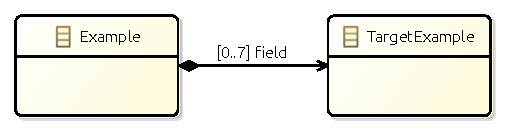
\includegraphics{images/05_library_of_transformations/02_type_level_transformations/10_contained_class_set_fields/contained_class_set_field.pdf}
        \caption{$Tm_{ContainedClassSetField}$ to a class type $.\type{TargetExample}$ with $name = \type{field}$}
        \label{fig:library_of_transformations:type_level_transformations:contained_class_set_fields:visualisation:ecore}
    \end{subfigure}
    \\
    \begin{subfigure}{0.95\textwidth}
        \centering
        % To use this figure in your LaTeX document
% import the package groove/resources/groove2tikz.sty
%
\begin{tikzpicture}[scale=\tikzscale,name prefix=test-]
\node[type_node] (n0) at (3.125, -0.945) {\ml{\textbf{Example}}};
\node[type_node] (n1) at (5.040, -0.950) {\ml{\textbf{TargetExample}}};

\path[basic_edge, composite](n0.east |- 5.040, -0.950) -- node[lab] {\ml{field}} (n1) ;
\end{tikzpicture}

        \caption{$TG_{ContainedClassSetField}$ to a class type $\type{TargetExample}$ with $name = \type{field}$}
        \label{fig:library_of_transformations:type_level_transformations:contained_class_set_fields:visualisation:groove}
    \end{subfigure}
    \caption{Visualisation of the transformation of a containment field typed by a set of a proper class type}
    \label{fig:library_of_transformations:type_level_transformations:contained_class_set_fields:visualisation}
\end{figure}

In this section, the transformation of a containment field typed by a set of a proper class type is shown. This transformation defines a field which has a value a set of objects of a specified class type, that is not nullable. Furthermore, the objects referenced by the field are contained by the source class. First, the Ecore type model is defined.

\begin{defin}[Type model $Tm_{ContainedClassSetField}$]
\label{defin:library_of_transformations:type_level_transformations:contained_class_set_fields:tmod_contained_class_set_field}
Let $Tm_{ContainedClassSetField}$ be the type model containing a regular class with identifier $classtype$. Then $Tm_{ContainedClassSetField}$ defines a field named $name$ with type $containedtype$, in which $containedtype$ is the identifier of another class type in $Tm_{ContainedClassSetField}$. Furthermore, define $mul$ to be a valid multiplicity for the field $name$. $Tm_{ContainedClassSetField}$ is defined as:
\begin{align*}
Class =\ &\{classtype, containedtype\} \\
Enum =\ &\{\} \\
UserDataType =\ &\{\} \\
Field =\ &\{(classtype, name)\} \\
\mathrm{FieldSig} =\ &\begin{cases}
    (f, ((\type{setof}, !containedtype), mul)) &\mathrm{if}\ f \in Field_{Tm_{ContainedClassSetField}}
\end{cases} \\
EnumValue =\ &\{\} \\
Inh =\ &\{\} \\
Prop =\ &\{(\type{containment}, (classtype, name))\} \\
Constant =\ &\{\} \\
\mathrm{ConstType} =\ &\{\}
\end{align*}
\isabellelref{tmod_contained_class_set_field}{Ecore-GROOVE-Mapping-Library.ContainedClassSetField}
\end{defin}

\begin{thm}[Correctness of $Tm_{ContainedClassSetField}$]
\label{defin:library_of_transformations:type_level_transformations:contained_class_set_fields:tmod_contained_class_set_field_correct}
$Tm_{ContainedClassSetField}$ (\cref{defin:library_of_transformations:type_level_transformations:contained_class_set_fields:tmod_contained_class_set_field}) is a consistent type model in the sense of \cref{defin:formalisations:ecore_formalisation:type_models:type_model_consistency}.
\isabellelref{tmod_contained_class_set_field_correct}{Ecore-GROOVE-Mapping-Library.ContainedClassSetField}
\end{thm}

A visual representation of $Tm_{ContainedClassSetField}$ with field name $\type{field}$ on class $.\type{Example}$ can be seen in \cref{fig:library_of_transformations:type_level_transformations:contained_class_set_fields:visualisation:ecore}. In this example, $\type{field}$ references a class of $.\type{TargetExample}$. Please note that the multiplicity $0..7$ has been chosen here as an example, any valid multiplicity could have been used. Also notice that the field is in fact a containment relation. The correctness proof of $Tm_{ContainedClassSetField}$ is more involved, it is not included here for conciseness. It can be found within the validated Isabelle proofs.

In order to make composing transformation functions possible, $Tm_{ContainedClassSetField}$ should be compatible with the type model it is combined with.

\begin{thm}[Correctness of $\mathrm{combine}(Tm, Tm_{ContainedClassSetField})$]
\label{defin:library_of_transformations:type_level_transformations:contained_class_set_fields:tmod_contained_class_set_field_combine_correct}
Assume a type model $Tm$ that is consistent in the sense of \cref{defin:formalisations:ecore_formalisation:type_models:type_model_consistency}. Then $Tm$ is compatible with $Tm_{ContainedClassSetField}$ (in the sense of \cref{defin:transformation_framework:type_models_and_type_graphs:combining_type_models:compatibility}) if:
\begin{itemize}
    \item The class type on which the field is defined, $classtype$, is already an existing class in $Tm$;
    \item The class type which the field targets, $containedtype$, is already an existing class in $Tm$;
    \item The field named $name$ is not already a field on $classtype$ in $Tm$;
    \item The multiplicity $mul$ is valid.
\end{itemize}
\isabellelref{tmod_contained_class_set_field_combine_correct}{Ecore-GROOVE-Mapping-Library.ContainedClassSetField}
\end{thm}

\begin{proof}
Use \cref{defin:transformation_framework:type_models_and_type_graphs:combining_type_models:tmod_combine_merge_correct}. It is possible to show that all assumptions hold. Now we have shown that $\mathrm{combine}(Tm, Tm_{ContainedClassSetField})$ is consistent in the sense of \cref{defin:formalisations:ecore_formalisation:type_models:type_model_consistency}.
\end{proof}

The definitions and theorems for defining a data field within Ecore are now complete. 

\subsubsection{Encoding as edge type}

Like the previous encodings of fields, an edge type in GROOVE will be used as encoding for the field. The field is transformed into an edge type from the encoded class type to the encoded target type. Furthermore, the edge type will be a containment edge, to support the fact that the target nodes are contained by the source nodes. The encoding corresponding to $Tm_{ContainedClassSetField}$ can then be represented as $TG_{ContainedClassSetField}$, defined in the following definition:

\begin{defin}[Type graph $TG_{ContainedClassSetField}$]
\label{defin:library_of_transformations:type_level_transformations:contained_class_set_fields:tg_contained_class_set_field_as_edge_type}
Let $TG_{ContainedClassSetField}$ be the type graph containing a node type which encodes the class type $classtype$. Furthermore, define an edge type from $classtype$ named $name$. This edge type targets a node of $containedtype$. Finally, define multiplicity $mul$ to be  $TG_{ContainedClassSetField}$ is defined as:
\begin{align*}
NT =\ &\{\mathrm{ns\_\!to\_\!list}(classtype), \mathrm{ns\_\!to\_\!list}(containedtype)\} \\
ET =\ &\{(\mathrm{ns\_\!to\_\!list}(classtype), \langle name \rangle, \mathrm{ns\_\!to\_\!list}(containedtype))\} \\
\!\!\sqsubseteq\ =\ &\{( \mathrm{ns\_\!to\_\!list}(classtype), \mathrm{ns\_\!to\_\!list}(classtype) ),\\&( \mathrm{ns\_\!to\_\!list}(containedtype), \mathrm{ns\_\!to\_\!list}(containedtype) )\} \\
abs =\ &\{\} \\
\mathrm{mult}(e) =\ &\begin{cases}
    (0..1, mul) &\mathrm{if}\ e \in \{(\mathrm{ns\_\!to\_\!list}(classtype), \langle name \rangle, \mathrm{ns\_\!to\_\!list}(containedtype))\}
\end{cases} \\
contains =\ &\{(\mathrm{ns\_\!to\_\!list}(classtype), \langle name \rangle, \mathrm{ns\_\!to\_\!list}(containedtype))\}
\end{align*}
\isabellelref{tg_contained_class_set_field_as_edge_type}{Ecore-GROOVE-Mapping-Library.ContainedClassSetField}
\end{defin}

\begin{thm}[Correctness of $TG_{ContainedClassSetField}$]
\label{defin:library_of_transformations:type_level_transformations:contained_class_set_fields:tg_contained_class_set_field_as_edge_type_correct}
$TG_{ContainedClassSetField}$ (\cref{defin:library_of_transformations:type_level_transformations:contained_class_set_fields:tg_contained_class_set_field_as_edge_type}) is a valid type graph in the sense of \cref{defin:formalisations:groove_formalisation:type_graphs:type_graph_validity}.
\isabellelref{tg_contained_class_set_field_as_edge_type_correct}{Ecore-GROOVE-Mapping-Library.ContainedClassSetField}
\end{thm}

A visual representation of $TG_{ContainedClassSetField}$ with edge name $\type{field}$ on node type $\type{Example}$ can be seen in \cref{fig:library_of_transformations:type_level_transformations:contained_class_set_fields:visualisation:groove}. Like the previous example, $\type{field}$ references the $.\type{TargetExample}$ class, but in this case the encoded node type of $\type{TargetExample}$. Furthermore, it is visable that the introduced edge type for the field is indeed a containment edge. The correctness proof of $TG_{ContainedClassSetField}$ is more involved, it is not included here for conciseness. It can be found within the validated Isabelle proofs.

In order to make composing transformation functions possible, $TG_{ContainedClassSetField}$ should be compatible with the type graph it is combined with.

\begin{thm}[Correctness of $\mathrm{combine}(TG, TG_{ContainedClassSetField})$]
\label{defin:library_of_transformations:type_level_transformations:contained_class_set_fields:tg_contained_class_set_field_as_edge_type_combine_correct}
Assume a type graph $TG$ that is valid in the sense of \cref{defin:formalisations:groove_formalisation:type_graphs:type_graph_validity}. Then $TG$ is compatible with $TG_{ContainedClassSetField}$ (in the sense of \cref{defin:transformation_framework:type_models_and_type_graphs:combining_type_graphs:compatibility}) if:
\begin{itemize}
    \item The node types of the encoded class types in $TG_{ContainedClassSetField}$ are already node types in $TG$.
    \item The node type of the encoded class type in $TG_{ContainedClassSetField}$ does not already have an edge type with the same name as the field in $TG$;
    \item The multiplicity $mul$ is valid.
\end{itemize}
\isabellelref{tg_contained_class_set_field_as_edge_type_combine_correct}{Ecore-GROOVE-Mapping-Library.ContainedClassSetField}
\end{thm}

\begin{proof}
Use \cref{defin:transformation_framework:type_models_and_type_graphs:combining_type_graphs:tg_combine_merge_correct}. It is possible to show that all assumptions hold. Now we have shown that $\mathrm{combine}(TG, TG_{ContainedClassSetField})$ is valid in the sense of \cref{defin:formalisations:groove_formalisation:type_graphs:type_graph_validity}.
\end{proof}

The next definitions define the transformation function from $Tm_{ContainedClassSetField}$ to $TG_{ContainedClassSetField}$:

\begin{defin}[Transformation function $f_{ContainedClassSetField}$]
\label{defin:library_of_transformations:type_level_transformations:contained_class_set_fields:tmod_contained_class_set_field_to_tg_contained_class_set_field_as_edge_type}
The transformation function $f_{ContainedClassSetField}(Tm)$ is defined as:
\begin{align*}
NT =\ &\{\mathrm{ns\_\!to\_\!list}(c) \mid c \in Class_{Tm}\}\\
ET =\ &\{(\mathrm{ns\_\!to\_\!list}(c), \langle f \rangle, \mathrm{ns\_\!to\_\!list}(containedtype)) \mid (c, n) \in Field_{Tm} \} \\
\!\!\sqsubseteq\ =\ &\{( \mathrm{ns\_\!to\_\!list}(c), \mathrm{ns\_\!to\_\!list}(c) ) \mid c \in Class_{Tm} \} \\
abs =\ &\{\} \\
\mathrm{mult} =\ &\begin{cases}
    (0..1, mul) &\mathrm{if}\ e \in \{(\mathrm{ns\_\!to\_\!list}(c), \langle f \rangle, \mathrm{ns\_\!to\_\!list}(containedtype)) \mid (c, n) \in Field_{Tm} \}
\end{cases} \\
contains =\ &\{(\mathrm{ns\_\!to\_\!list}(c), \langle f \rangle, \mathrm{ns\_\!to\_\!list}(containedtype)) \mid (c, n) \in Field_{Tm} \}
\end{align*}
\isabellelref{tmod_contained_class_set_field_to_tg_contained_class_set_field_as_edge_type}{Ecore-GROOVE-Mapping-Library.ContainedClassSetField}
\end{defin}

\begin{thm}[Correctness of $f_{ContainedClassSetField}$]
\label{defin:library_of_transformations:type_level_transformations:contained_class_set_fields:tmod_contained_class_set_field_to_tg_contained_class_set_field_as_edge_type_func}
$f_{ContainedClassSetField}(Tm)$ (\cref{defin:library_of_transformations:type_level_transformations:contained_class_set_fields:tmod_contained_class_set_field_to_tg_contained_class_set_field_as_edge_type}) is a valid transformation function in the sense of \cref{defin:transformation_framework:type_models_and_type_graphs:combining_transformation_functions:transformation_function_type_model_type_graph} transforming $Tm_{ContainedClassSetField}$ into $TG_{ContainedClassSetField}$.
\isabellelref{tmod_contained_class_set_field_to_tg_contained_class_set_field_as_edge_type_func}{Ecore-GROOVE-Mapping-Library.ContainedClassSetField}
\end{thm}

The proof of the correctness of $f_{ContainedClassSetField}$ will not be included here. Instead, it can be found in the validated Isabelle theories.

Finally, to complete the transformation, the transformation function that transforms $TG_{ContainedClassSetField}$ into $Tm_{ContainedClassSetField}$ is defined:

\begin{defin}[Transformation function $f'_{ContainedClassSetField}$]
\label{defin:library_of_transformations:type_level_transformations:contained_class_set_fields:tg_contained_class_set_field_as_edge_type_to_tmod_contained_class_set_field}
The transformation function $f'_{ContainedClassSetField}(TG)$ is defined as:
\begin{align*}
Class =\ &\{\mathrm{list\_\!to\_\!ns}(n) \mid n \in NT_{TG} \} \\
Enum =\ &\{\} \\
UserDataType =\ &\{\} \\
Field =\ &\{(\mathrm{list\_\!to\_\!ns}(\mathrm{src}(e)), l) \mid e \in ET_{TG} \land \langle l \rangle = \mathrm{lab}(e) \} \\
\mathrm{FieldSig} =\ &\begin{cases}
    (f, ((\type{setof}, !containedtype), mul)) &\mathrm{if}\ f \in \{(\mathrm{list\_\!to\_\!ns}(\mathrm{src}(e)), l) \mid e \in ET_{TG}\ \land\\&\qquad\quad \langle l \rangle = \mathrm{lab}(e) \} 
\end{cases} \\
EnumValue =\ &\{\} \\
Inh =\ &\{\} \\
Prop =\ &\{(\type{containment}, (\mathrm{list\_\!to\_\!ns}(\mathrm{src}(e)), l)) \mid e \in ET_{TG} \land \langle l \rangle = \mathrm{lab}(e) \} \\
Constant =\ &\{\} \\
\mathrm{ConstType} =\ &\{\}
\end{align*}
\isabellelref{tg_contained_class_set_field_as_edge_type_to_tmod_contained_class_set_field}{Ecore-GROOVE-Mapping-Library.ContainedClassSetField}
\end{defin}

\begin{thm}[Correctness of $f'_{ContainedClassSetField}$]
\label{defin:library_of_transformations:type_level_transformations:contained_class_set_fields:tg_contained_class_set_field_as_edge_type_to_tmod_contained_class_set_field_func}
$f'_{ContainedClassSetField}(TG)$ (\cref{defin:library_of_transformations:type_level_transformations:contained_class_set_fields:tg_contained_class_set_field_as_edge_type_to_tmod_contained_class_set_field}) is a valid transformation function in the sense of \cref{defin:transformation_framework:type_models_and_type_graphs:combining_transformation_functions:transformation_function_type_graph_type_model} transforming $TG_{ContainedClassSetField}$ into $Tm_{ContainedClassSetField}$.
\isabellelref{tg_contained_class_set_field_as_edge_type_to_tmod_contained_class_set_field_func}{Ecore-GROOVE-Mapping-Library.ContainedClassSetField}
\end{thm}

Once more, the correctness proof is not included here but can be found in the validated Isabelle proofs of this thesis.